% Options for packages loaded elsewhere
\PassOptionsToPackage{unicode}{hyperref}
\PassOptionsToPackage{hyphens}{url}
%
\documentclass[
]{article}
\usepackage{lmodern}
\usepackage{amssymb,amsmath}
\usepackage{ifxetex,ifluatex}
\ifnum 0\ifxetex 1\fi\ifluatex 1\fi=0 % if pdftex
  \usepackage[T1]{fontenc}
  \usepackage[utf8]{inputenc}
  \usepackage{textcomp} % provide euro and other symbols
\else % if luatex or xetex
  \usepackage{unicode-math}
  \defaultfontfeatures{Scale=MatchLowercase}
  \defaultfontfeatures[\rmfamily]{Ligatures=TeX,Scale=1}
\fi
% Use upquote if available, for straight quotes in verbatim environments
\IfFileExists{upquote.sty}{\usepackage{upquote}}{}
\IfFileExists{microtype.sty}{% use microtype if available
  \usepackage[]{microtype}
  \UseMicrotypeSet[protrusion]{basicmath} % disable protrusion for tt fonts
}{}
\makeatletter
\@ifundefined{KOMAClassName}{% if non-KOMA class
  \IfFileExists{parskip.sty}{%
    \usepackage{parskip}
  }{% else
    \setlength{\parindent}{0pt}
    \setlength{\parskip}{6pt plus 2pt minus 1pt}}
}{% if KOMA class
  \KOMAoptions{parskip=half}}
\makeatother
\usepackage{xcolor}
\IfFileExists{xurl.sty}{\usepackage{xurl}}{} % add URL line breaks if available
\IfFileExists{bookmark.sty}{\usepackage{bookmark}}{\usepackage{hyperref}}
\hypersetup{
  pdftitle={seshat\_epoques},
  pdfauthor={Achille-Laurent},
  hidelinks,
  pdfcreator={LaTeX via pandoc}}
\urlstyle{same} % disable monospaced font for URLs
\usepackage[margin=1in]{geometry}
\usepackage{color}
\usepackage{fancyvrb}
\newcommand{\VerbBar}{|}
\newcommand{\VERB}{\Verb[commandchars=\\\{\}]}
\DefineVerbatimEnvironment{Highlighting}{Verbatim}{commandchars=\\\{\}}
% Add ',fontsize=\small' for more characters per line
\usepackage{framed}
\definecolor{shadecolor}{RGB}{248,248,248}
\newenvironment{Shaded}{\begin{snugshade}}{\end{snugshade}}
\newcommand{\AlertTok}[1]{\textcolor[rgb]{0.94,0.16,0.16}{#1}}
\newcommand{\AnnotationTok}[1]{\textcolor[rgb]{0.56,0.35,0.01}{\textbf{\textit{#1}}}}
\newcommand{\AttributeTok}[1]{\textcolor[rgb]{0.77,0.63,0.00}{#1}}
\newcommand{\BaseNTok}[1]{\textcolor[rgb]{0.00,0.00,0.81}{#1}}
\newcommand{\BuiltInTok}[1]{#1}
\newcommand{\CharTok}[1]{\textcolor[rgb]{0.31,0.60,0.02}{#1}}
\newcommand{\CommentTok}[1]{\textcolor[rgb]{0.56,0.35,0.01}{\textit{#1}}}
\newcommand{\CommentVarTok}[1]{\textcolor[rgb]{0.56,0.35,0.01}{\textbf{\textit{#1}}}}
\newcommand{\ConstantTok}[1]{\textcolor[rgb]{0.00,0.00,0.00}{#1}}
\newcommand{\ControlFlowTok}[1]{\textcolor[rgb]{0.13,0.29,0.53}{\textbf{#1}}}
\newcommand{\DataTypeTok}[1]{\textcolor[rgb]{0.13,0.29,0.53}{#1}}
\newcommand{\DecValTok}[1]{\textcolor[rgb]{0.00,0.00,0.81}{#1}}
\newcommand{\DocumentationTok}[1]{\textcolor[rgb]{0.56,0.35,0.01}{\textbf{\textit{#1}}}}
\newcommand{\ErrorTok}[1]{\textcolor[rgb]{0.64,0.00,0.00}{\textbf{#1}}}
\newcommand{\ExtensionTok}[1]{#1}
\newcommand{\FloatTok}[1]{\textcolor[rgb]{0.00,0.00,0.81}{#1}}
\newcommand{\FunctionTok}[1]{\textcolor[rgb]{0.00,0.00,0.00}{#1}}
\newcommand{\ImportTok}[1]{#1}
\newcommand{\InformationTok}[1]{\textcolor[rgb]{0.56,0.35,0.01}{\textbf{\textit{#1}}}}
\newcommand{\KeywordTok}[1]{\textcolor[rgb]{0.13,0.29,0.53}{\textbf{#1}}}
\newcommand{\NormalTok}[1]{#1}
\newcommand{\OperatorTok}[1]{\textcolor[rgb]{0.81,0.36,0.00}{\textbf{#1}}}
\newcommand{\OtherTok}[1]{\textcolor[rgb]{0.56,0.35,0.01}{#1}}
\newcommand{\PreprocessorTok}[1]{\textcolor[rgb]{0.56,0.35,0.01}{\textit{#1}}}
\newcommand{\RegionMarkerTok}[1]{#1}
\newcommand{\SpecialCharTok}[1]{\textcolor[rgb]{0.00,0.00,0.00}{#1}}
\newcommand{\SpecialStringTok}[1]{\textcolor[rgb]{0.31,0.60,0.02}{#1}}
\newcommand{\StringTok}[1]{\textcolor[rgb]{0.31,0.60,0.02}{#1}}
\newcommand{\VariableTok}[1]{\textcolor[rgb]{0.00,0.00,0.00}{#1}}
\newcommand{\VerbatimStringTok}[1]{\textcolor[rgb]{0.31,0.60,0.02}{#1}}
\newcommand{\WarningTok}[1]{\textcolor[rgb]{0.56,0.35,0.01}{\textbf{\textit{#1}}}}
\usepackage{graphicx,grffile}
\makeatletter
\def\maxwidth{\ifdim\Gin@nat@width>\linewidth\linewidth\else\Gin@nat@width\fi}
\def\maxheight{\ifdim\Gin@nat@height>\textheight\textheight\else\Gin@nat@height\fi}
\makeatother
% Scale images if necessary, so that they will not overflow the page
% margins by default, and it is still possible to overwrite the defaults
% using explicit options in \includegraphics[width, height, ...]{}
\setkeys{Gin}{width=\maxwidth,height=\maxheight,keepaspectratio}
% Set default figure placement to htbp
\makeatletter
\def\fps@figure{htbp}
\makeatother
\setlength{\emergencystretch}{3em} % prevent overfull lines
\providecommand{\tightlist}{%
  \setlength{\itemsep}{0pt}\setlength{\parskip}{0pt}}
\setcounter{secnumdepth}{-\maxdimen} % remove section numbering

\title{seshat\_epoques}
\author{Achille-Laurent}
\date{03/06/2020}

\begin{document}
\maketitle

\hypertarget{analyse-uxe0-diffuxe9rentes-uxe9poques}{%
\section{3 Analyse à différentes
époques}\label{analyse-uxe0-diffuxe9rentes-uxe9poques}}

Code concernant la partie de l'analyse à différentes époques

\begin{Shaded}
\begin{Highlighting}[]
\NormalTok{dfn <-}\StringTok{ }\KeywordTok{read.csv}\NormalTok{(}\StringTok{'../databases/axial.csv'}\NormalTok{,}\DataTypeTok{sep=}\StringTok{','}\NormalTok{) }\CommentTok{#NGA et Time séparés sur deux colonnes}
\NormalTok{dfn_melange <-}\StringTok{ }\KeywordTok{read.csv}\NormalTok{(}\StringTok{'../databases/axial_index.csv'}\NormalTok{,}\DataTypeTok{sep=}\StringTok{','}\NormalTok{) }\CommentTok{#contient une colonne regroupant NGA et Time}
\NormalTok{pays_et_date =}\StringTok{ }\NormalTok{dfn_melange[[}\DecValTok{1}\NormalTok{]]}
\NormalTok{dfn[[}\DecValTok{1}\NormalTok{]] =}\StringTok{ }\NormalTok{pays_et_date}
\KeywordTok{colnames}\NormalTok{(dfn)}
\end{Highlighting}
\end{Shaded}

\begin{verbatim}
##  [1] "NGA"        "PolID"      "Time"       "PolPop"     "PolTerr"   
##  [6] "CapPop"     "levels"     "government" "infrastr"   "writing"   
## [11] "texts"      "money"      "SPC1"       "MG_corr"
\end{verbatim}

\begin{Shaded}
\begin{Highlighting}[]
\KeywordTok{colnames}\NormalTok{(dfn_melange)}
\end{Highlighting}
\end{Shaded}

\begin{verbatim}
##  [1] "Index"      "NGA"        "PolID"      "Time"       "PolPop"    
##  [6] "PolTerr"    "CapPop"     "levels"     "government" "infrastr"  
## [11] "writing"    "texts"      "money"
\end{verbatim}

\begin{Shaded}
\begin{Highlighting}[]
\KeywordTok{length}\NormalTok{(}\KeywordTok{colnames}\NormalTok{(dfn))}
\end{Highlighting}
\end{Shaded}

\begin{verbatim}
## [1] 14
\end{verbatim}

\begin{Shaded}
\begin{Highlighting}[]
\KeywordTok{rownames}\NormalTok{(dfn) <-}\StringTok{ }\NormalTok{dfn}\OperatorTok{$}\NormalTok{NGA}
\NormalTok{dfn =}\StringTok{ }\KeywordTok{subset}\NormalTok{(dfn, }\DataTypeTok{select=}\OperatorTok{-}\KeywordTok{c}\NormalTok{(PolID, SPC1, MG_corr, NGA))}
\KeywordTok{attach}\NormalTok{(dfn)}
\KeywordTok{head}\NormalTok{(dfn)}
\end{Highlighting}
\end{Shaded}

\begin{verbatim}
##                     Time   PolPop  PolTerr   CapPop     levels government
## Konya Plain (-9600) 1000 3.854914 4.111759 2.282858 -0.6537767 0.09090909
## Konya Plain (-9500) 1100 3.854914 4.111759 2.282858 -0.6537767 0.09090909
## Konya Plain (-9400) 1200 3.750606 3.337475 3.363416  1.0606111 0.09090909
## Konya Plain (-9300) 1300 4.065673 3.337475 3.429545  0.9434101 0.09090909
## Konya Plain (-9200) 1400 4.192464 3.337475 3.584463  1.9931297 0.09090909
## Konya Plain (-9100) 1500 4.599847 3.337475 3.807048  4.5642357 0.17272727
##                       infrastr writing texts money
## Konya Plain (-9600) 0.10000000    0.10   0.1   1.8
## Konya Plain (-9500) 0.10000000    0.10   0.1   1.8
## Konya Plain (-9400) 0.09090909    0.15   0.0   1.8
## Konya Plain (-9300) 0.09090909    0.15   0.0   1.8
## Konya Plain (-9200) 0.18181818    0.15   0.0   1.8
## Konya Plain (-9100) 0.18181818    0.15   0.0   1.8
\end{verbatim}

\begin{Shaded}
\begin{Highlighting}[]
\KeywordTok{head}\NormalTok{(dfn_melange)}
\end{Highlighting}
\end{Shaded}

\begin{verbatim}
##                 Index         NGA   PolID  Time   PolPop  PolTerr   CapPop
## 1 Konya Plain (-9600) Konya Plain TrNeoER -9600 3.293724 4.138263 1.442118
## 2 Konya Plain (-9500) Konya Plain TrNeoER -9500 3.293724 4.138263 1.442118
## 3 Konya Plain (-9400) Konya Plain TrNeoER -9400 3.293724 4.138263 1.442118
## 4 Konya Plain (-9300) Konya Plain TrNeoER -9300 3.293724 4.138263 1.442118
## 5 Konya Plain (-9200) Konya Plain TrNeoER -9200 3.293724 4.138263 1.442118
## 6 Konya Plain (-9100) Konya Plain TrNeoER -9100 3.293724 4.138263 1.442118
##        levels government infrastr writing texts money
## 1 -0.05581711          0        0       0     0     0
## 2 -0.05581711          0        0       0     0     0
## 3 -0.05581711          0        0       0     0     0
## 4 -0.05581711          0        0       0     0     0
## 5 -0.05581711          0        0       0     0     0
## 6 -0.05581711          0        0       0     0     0
\end{verbatim}

\begin{Shaded}
\begin{Highlighting}[]
\KeywordTok{str}\NormalTok{(dfn)}
\end{Highlighting}
\end{Shaded}

\begin{verbatim}
## 'data.frame':    864 obs. of  10 variables:
##  $ Time      : int  1000 1100 1200 1300 1400 1500 1600 1700 1800 -600 ...
##  $ PolPop    : num  3.85 3.85 3.75 4.07 4.19 ...
##  $ PolTerr   : num  4.11 4.11 3.34 3.34 3.34 ...
##  $ CapPop    : num  2.28 2.28 3.36 3.43 3.58 ...
##  $ levels    : num  -0.654 -0.654 1.061 0.943 1.993 ...
##  $ government: num  0.0909 0.0909 0.0909 0.0909 0.0909 ...
##  $ infrastr  : num  0.1 0.1 0.0909 0.0909 0.1818 ...
##  $ writing   : num  0.1 0.1 0.15 0.15 0.15 ...
##  $ texts     : num  0.1 0.1 0 0 0 0 0 0 0 0 ...
##  $ money     : num  1.8 1.8 1.8 1.8 1.8 1.8 1.8 1.8 1.8 1 ...
\end{verbatim}

\begin{itemize}
\tightlist
\item
  On répartit les données sur 3 époques, un jeu de données de taille
  environ 288 pour chaque époque \# t =
  table(dfn\(Time) # print(t) # cumsum(t) # head(dfn) # t2 = table(dfn\)NGA)
  \# names(t2)\\
  \# print(t2{[}t2\textless9{]}) \# length(t2{[}t2\textless9{]})
\end{itemize}

\begin{Shaded}
\begin{Highlighting}[]
\NormalTok{df1 =}\StringTok{ }\KeywordTok{subset}\NormalTok{(dfn, }\DecValTok{-9600} \OperatorTok{<=}\StringTok{ }\NormalTok{dfn}\OperatorTok{$}\NormalTok{Time }\OperatorTok{&}\StringTok{ }\NormalTok{dfn}\OperatorTok{$}\NormalTok{Time }\OperatorTok{<=}\StringTok{ }\DecValTok{-2100}\NormalTok{) }\CommentTok{#len = 288}
\NormalTok{df2 =}\StringTok{ }\KeywordTok{subset}\NormalTok{(dfn, }\DecValTok{-2000} \OperatorTok{<=}\StringTok{ }\NormalTok{dfn}\OperatorTok{$}\NormalTok{Time }\OperatorTok{&}\StringTok{ }\NormalTok{dfn}\OperatorTok{$}\NormalTok{Time }\OperatorTok{<=}\StringTok{ }\DecValTok{400}\NormalTok{) }\CommentTok{#len = 296}
\NormalTok{df3 =}\StringTok{ }\KeywordTok{subset}\NormalTok{(dfn, }\DecValTok{500} \OperatorTok{<=}\StringTok{ }\NormalTok{dfn}\OperatorTok{$}\NormalTok{Time }\OperatorTok{&}\StringTok{ }\NormalTok{dfn}\OperatorTok{$}\NormalTok{Time }\OperatorTok{<=}\StringTok{ }\DecValTok{1900}\NormalTok{) }\CommentTok{#len = 280}
\NormalTok{df1 =}\StringTok{ }\KeywordTok{subset}\NormalTok{(df1, }\DataTypeTok{select=}\OperatorTok{-}\KeywordTok{c}\NormalTok{(Time))}
\NormalTok{df2 =}\StringTok{ }\KeywordTok{subset}\NormalTok{(df2, }\DataTypeTok{select=}\OperatorTok{-}\KeywordTok{c}\NormalTok{(Time))}
\NormalTok{df3 =}\StringTok{ }\KeywordTok{subset}\NormalTok{(df3, }\DataTypeTok{select=}\OperatorTok{-}\KeywordTok{c}\NormalTok{(Time))}
\KeywordTok{head}\NormalTok{(df1)}
\end{Highlighting}
\end{Shaded}

\begin{verbatim}
##                       PolPop  PolTerr   CapPop    levels government infrastr
## Susiana (-5800)     2.731672 2.649571 3.150524 0.6666667        0.1    0.175
## Kachi Plain (-5800) 2.731672 2.649571 3.150524 0.6666667        0.1    0.175
## Konya Plain (-5700) 2.731672 2.649571 3.150524 0.6666667        0.1    0.175
## Susiana (-5700)     2.731672 2.649571 3.150524 0.6666667        0.1    0.175
## Kachi Plain (-5700) 2.731672 2.649571 3.150524 0.6666667        0.1    0.175
## Susiana (-5600)     2.731672 2.649571 3.150524 0.6666667        0.1    0.175
##                     writing texts money
## Susiana (-5800)         0.1   0.1   0.9
## Kachi Plain (-5800)     0.1   0.1   0.9
## Konya Plain (-5700)     0.1   0.1   0.9
## Susiana (-5700)         0.1   0.1   0.9
## Kachi Plain (-5700)     0.1   0.1   0.9
## Susiana (-5600)         0.1   0.1   0.9
\end{verbatim}

\hypertarget{vue-densemble}{%
\subsubsection{3.1. Vue d'ensemble}\label{vue-densemble}}

\begin{itemize}
\tightlist
\item
  boxplot
\end{itemize}

\begin{Shaded}
\begin{Highlighting}[]
\CommentTok{# Séparer les 2 plots qui sont d'échelle différente}
\KeywordTok{boxplot}\NormalTok{(}\DataTypeTok{main=}\StringTok{"df1"}\NormalTok{, }\KeywordTok{subset}\NormalTok{(df1,}\DataTypeTok{select =} \KeywordTok{c}\NormalTok{(PolPop,PolTerr,CapPop,levels,money)))}
\end{Highlighting}
\end{Shaded}

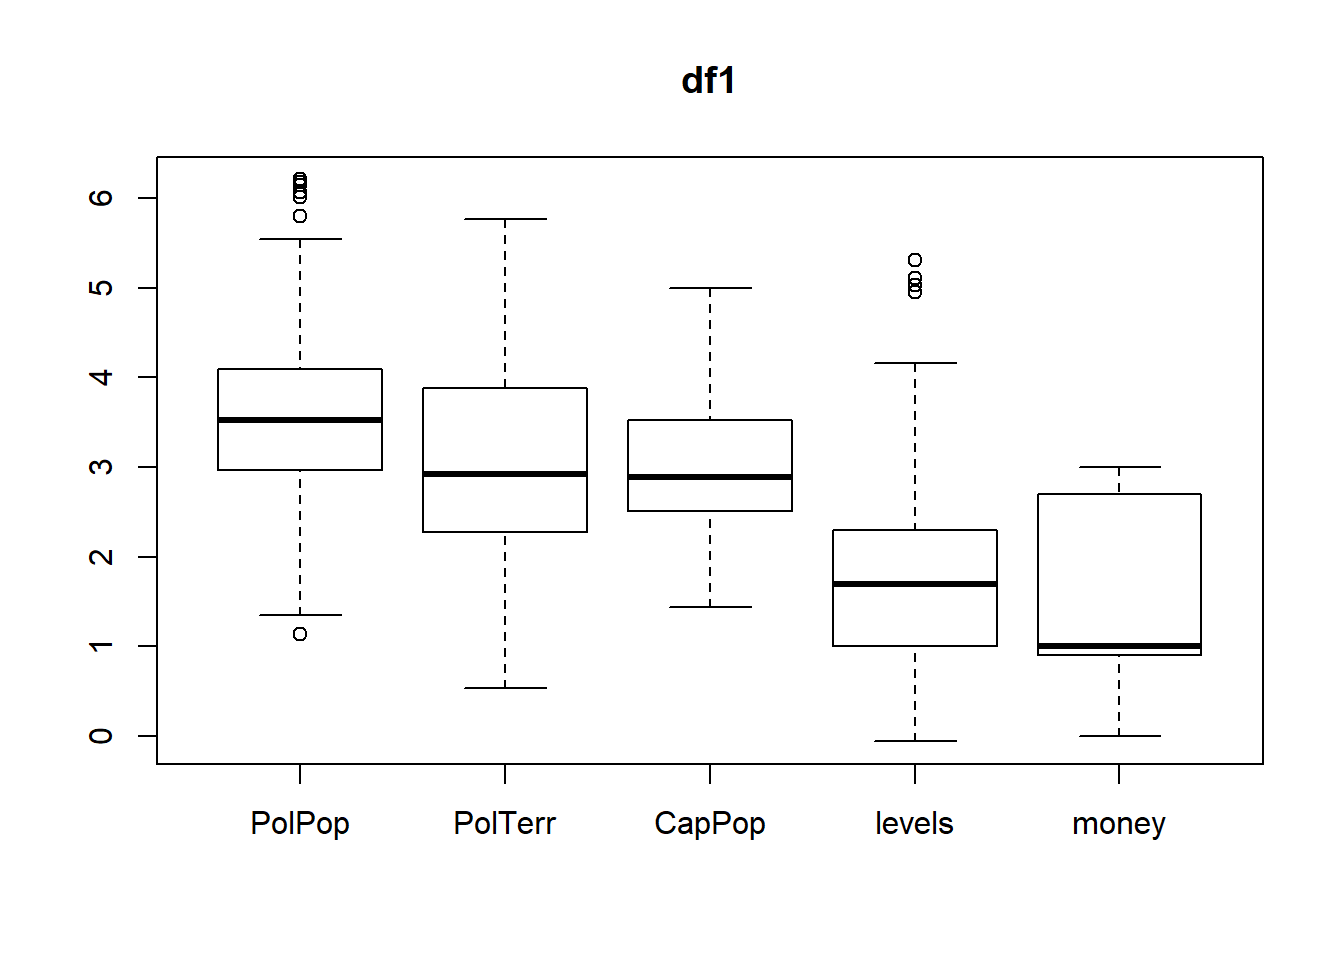
\includegraphics{seshat_laurent_files/figure-latex/unnamed-chunk-3-1.pdf}

\begin{Shaded}
\begin{Highlighting}[]
\KeywordTok{boxplot}\NormalTok{(}\DataTypeTok{main=}\StringTok{"df1"}\NormalTok{, }\KeywordTok{subset}\NormalTok{(df1,}\DataTypeTok{select =} \KeywordTok{c}\NormalTok{(government,infrastr,writing,texts)))}
\end{Highlighting}
\end{Shaded}

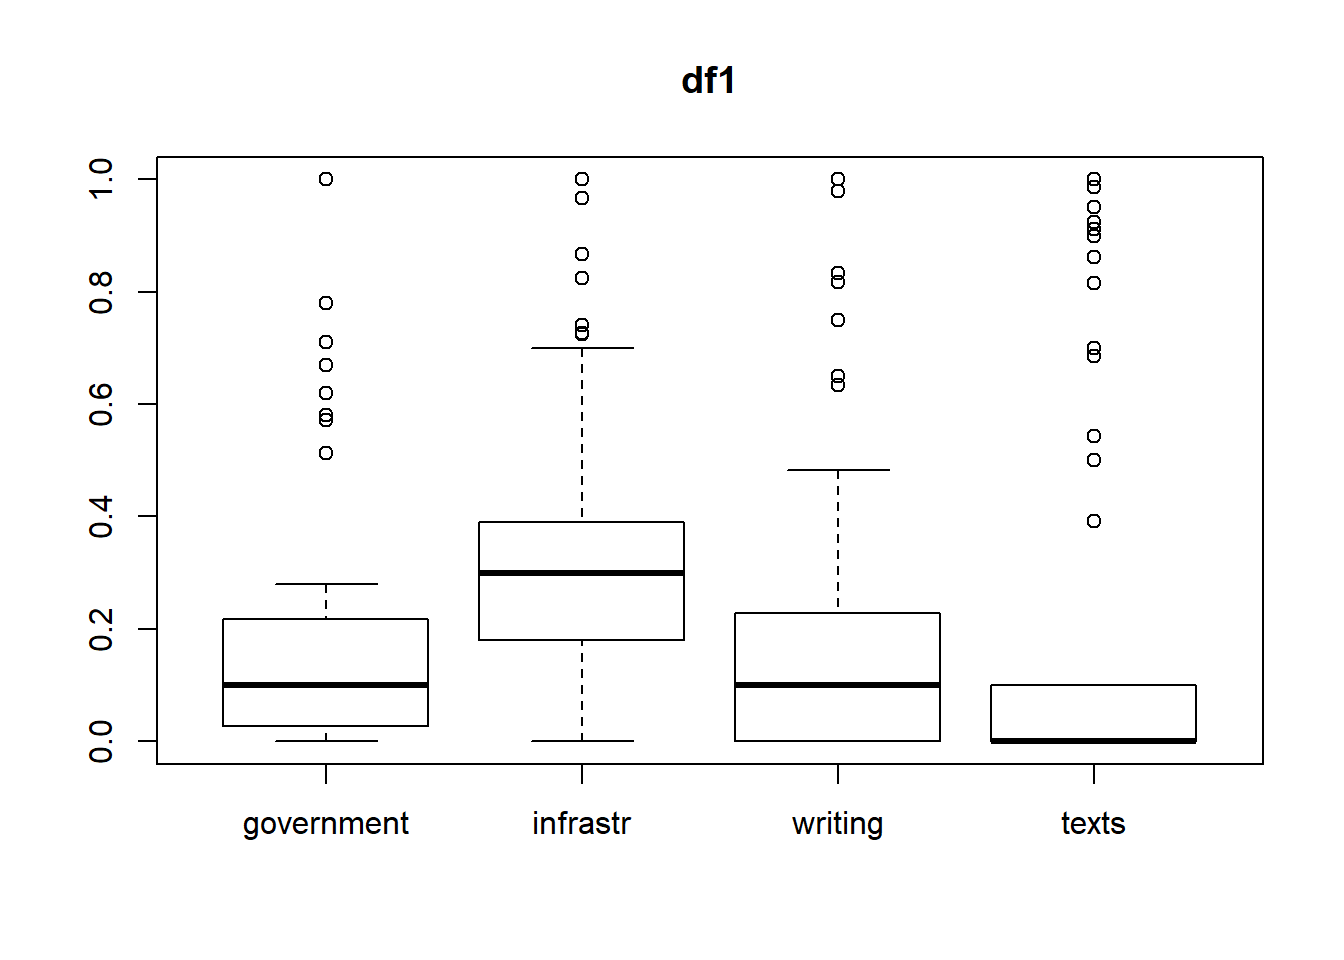
\includegraphics{seshat_laurent_files/figure-latex/unnamed-chunk-3-2.pdf}

\begin{Shaded}
\begin{Highlighting}[]
\KeywordTok{boxplot}\NormalTok{(}\DataTypeTok{main=}\StringTok{"df2"}\NormalTok{, }\KeywordTok{subset}\NormalTok{(df2,}\DataTypeTok{select =} \KeywordTok{c}\NormalTok{(PolPop,PolTerr,CapPop,levels,money)))}
\end{Highlighting}
\end{Shaded}

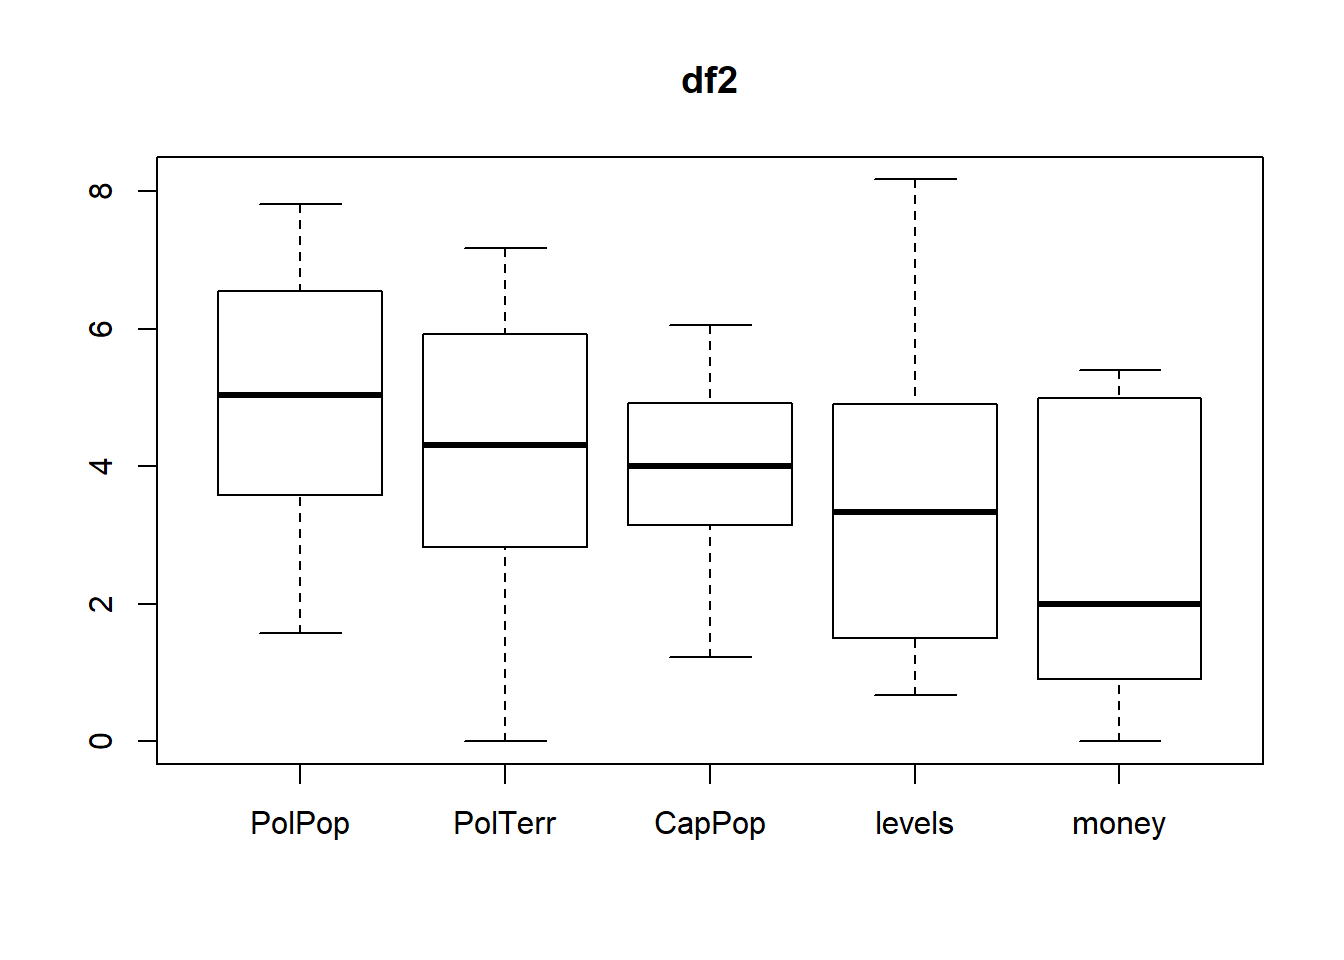
\includegraphics{seshat_laurent_files/figure-latex/unnamed-chunk-3-3.pdf}

\begin{Shaded}
\begin{Highlighting}[]
\KeywordTok{boxplot}\NormalTok{(}\DataTypeTok{main=}\StringTok{"df2"}\NormalTok{, }\KeywordTok{subset}\NormalTok{(df2,}\DataTypeTok{select =} \KeywordTok{c}\NormalTok{(government,infrastr,writing,texts)))}
\end{Highlighting}
\end{Shaded}

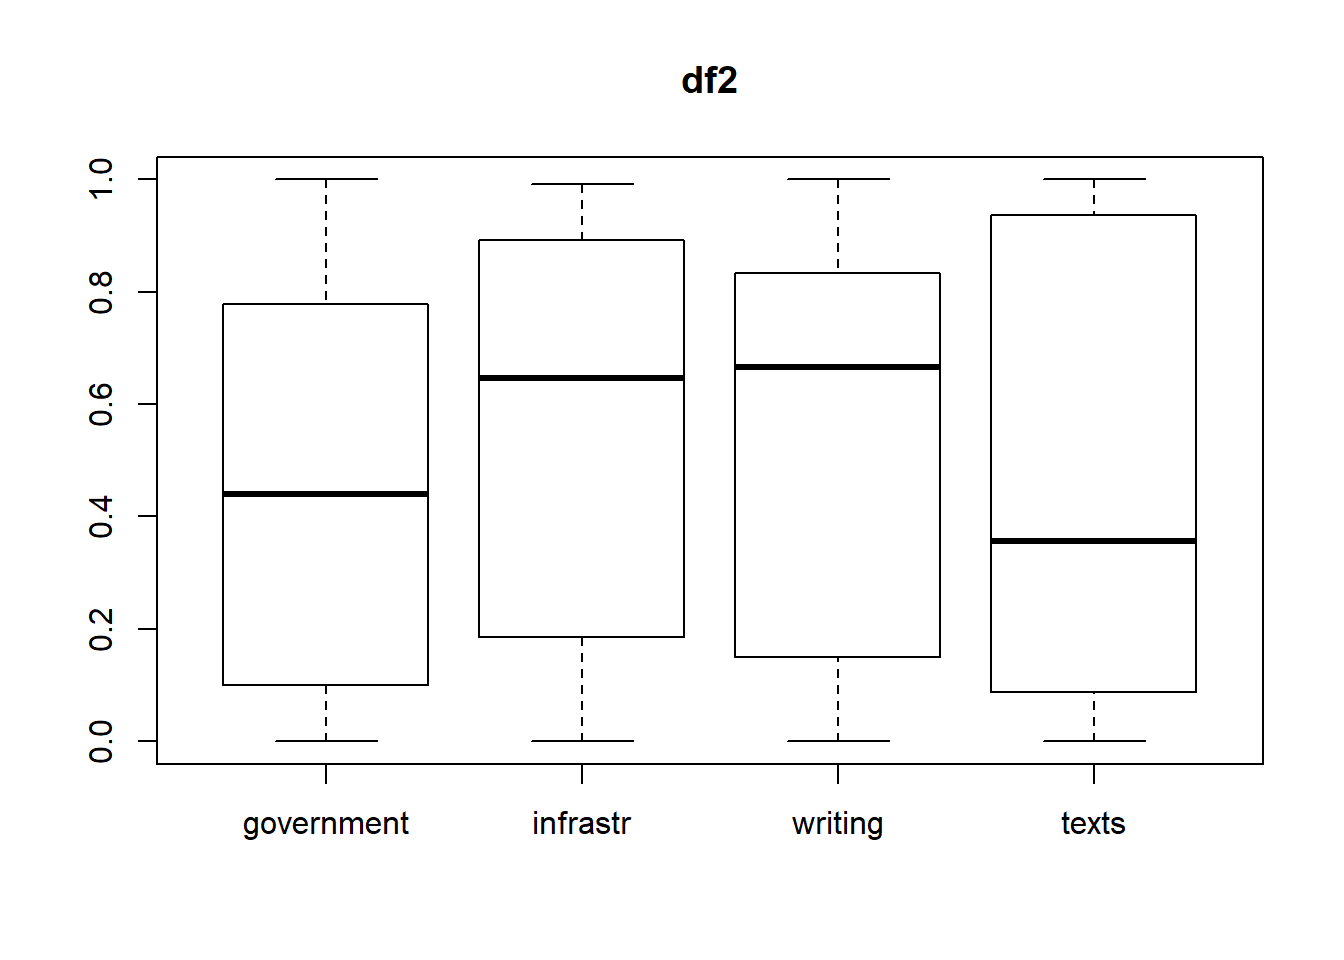
\includegraphics{seshat_laurent_files/figure-latex/unnamed-chunk-3-4.pdf}

\begin{Shaded}
\begin{Highlighting}[]
\KeywordTok{boxplot}\NormalTok{(}\DataTypeTok{main=}\StringTok{"df3"}\NormalTok{, }\KeywordTok{subset}\NormalTok{(df3,}\DataTypeTok{select =} \KeywordTok{c}\NormalTok{(PolPop,PolTerr,CapPop,levels,money)))}
\end{Highlighting}
\end{Shaded}

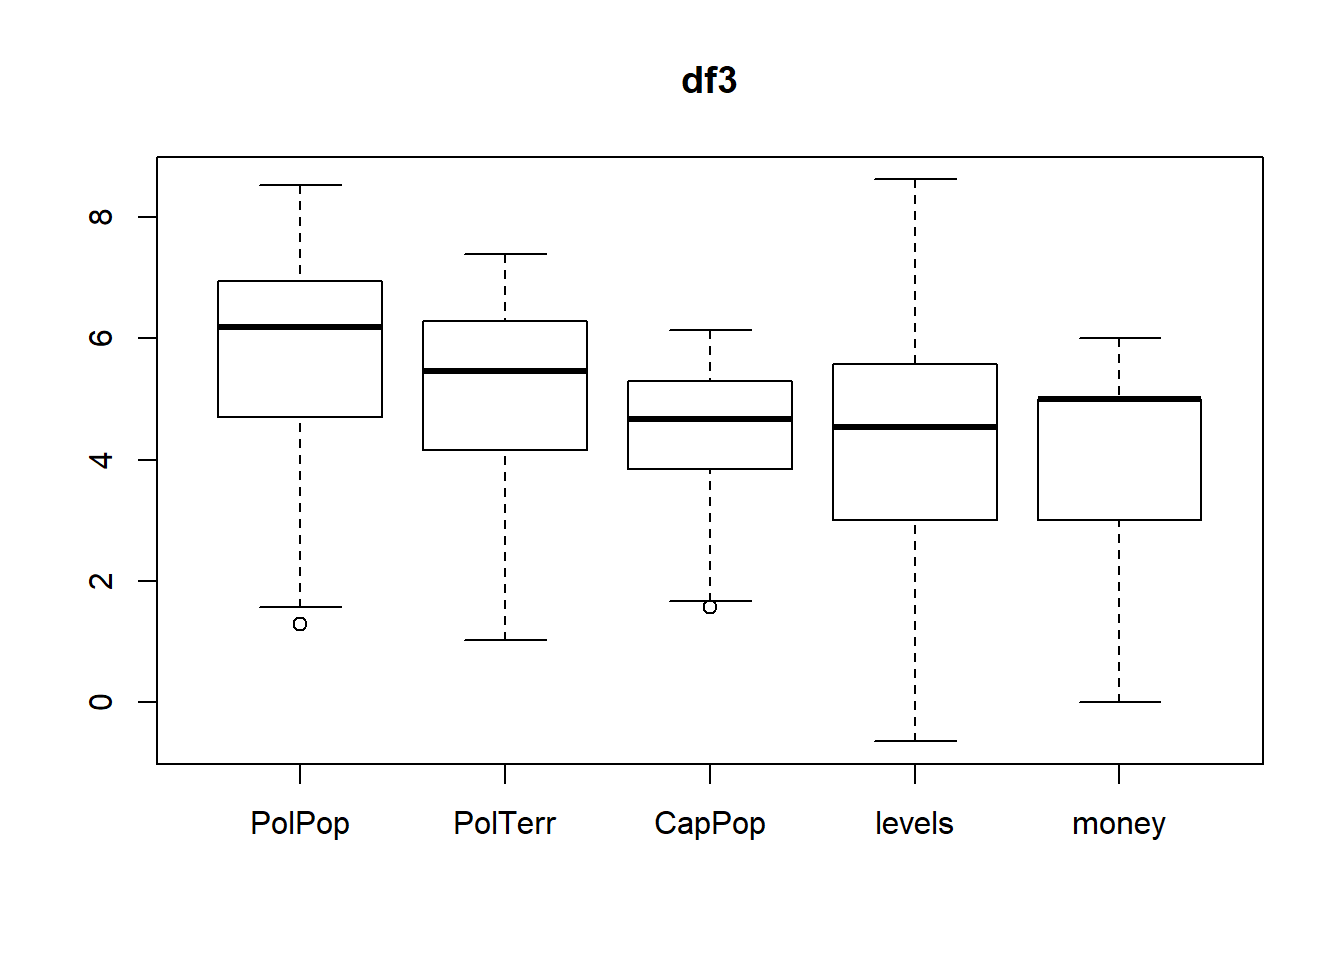
\includegraphics{seshat_laurent_files/figure-latex/unnamed-chunk-3-5.pdf}

\begin{Shaded}
\begin{Highlighting}[]
\KeywordTok{boxplot}\NormalTok{(}\DataTypeTok{main=}\StringTok{"df3"}\NormalTok{, }\KeywordTok{subset}\NormalTok{(df3,}\DataTypeTok{select =} \KeywordTok{c}\NormalTok{(government,infrastr,writing,texts)))}
\end{Highlighting}
\end{Shaded}

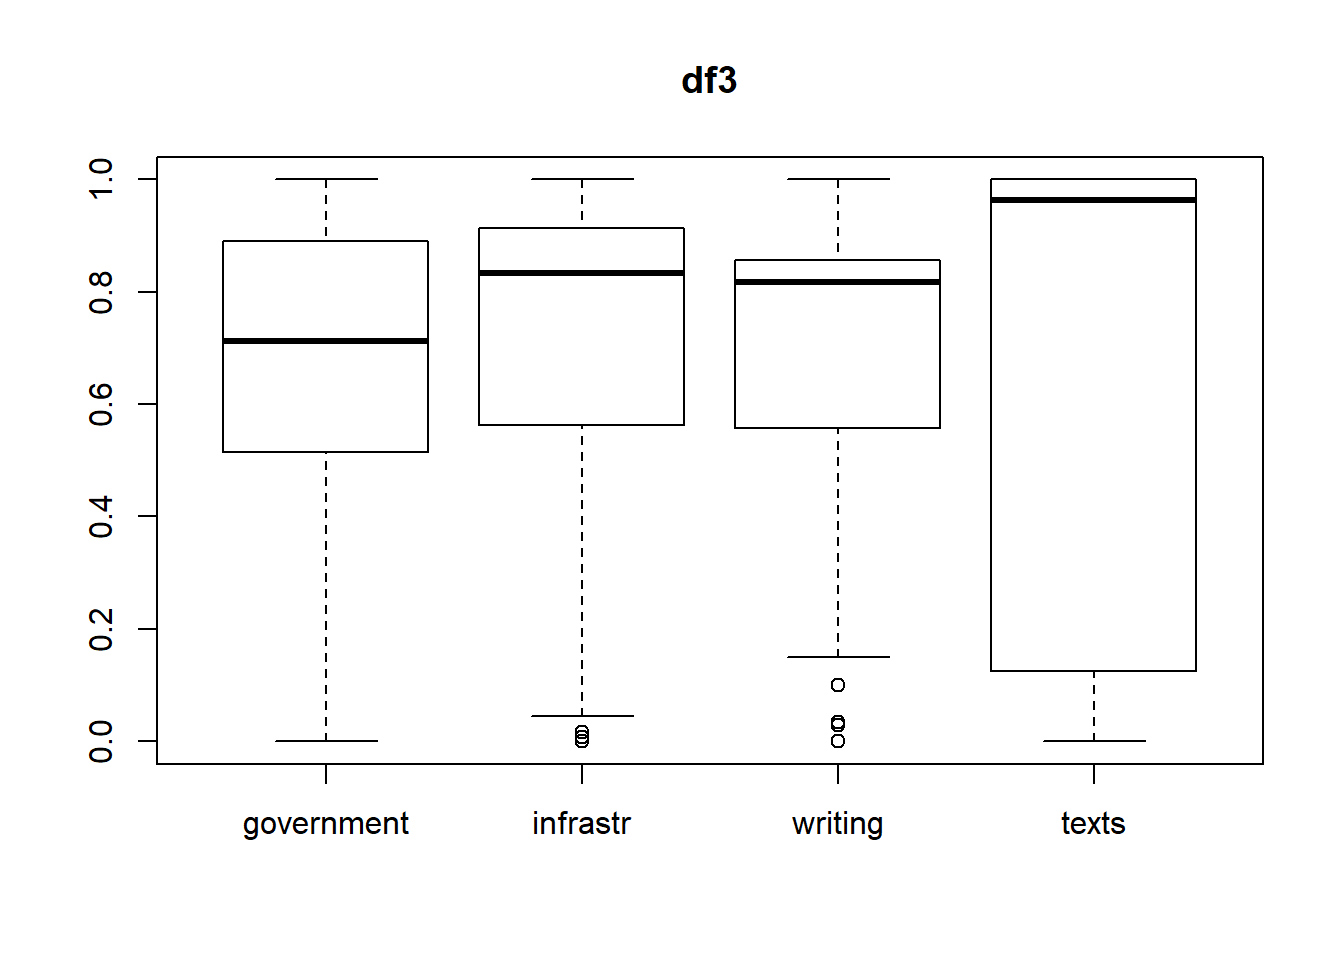
\includegraphics{seshat_laurent_files/figure-latex/unnamed-chunk-3-6.pdf}

\hypertarget{acp}{%
\subsubsection{3.2. ACP}\label{acp}}

\begin{itemize}
\tightlist
\item
  (2D, Prop Variance)
\end{itemize}

\begin{Shaded}
\begin{Highlighting}[]
\KeywordTok{typeof}\NormalTok{(df1)}
\end{Highlighting}
\end{Shaded}

\begin{verbatim}
## [1] "list"
\end{verbatim}

\begin{Shaded}
\begin{Highlighting}[]
\NormalTok{X1=}\StringTok{ }\KeywordTok{scale}\NormalTok{(df1, }\DataTypeTok{center=}\NormalTok{T, }\DataTypeTok{scale=}\NormalTok{T)}
\NormalTok{X2=}\StringTok{ }\KeywordTok{scale}\NormalTok{(df2, }\DataTypeTok{center=}\NormalTok{T, }\DataTypeTok{scale=}\NormalTok{T)}
\NormalTok{X3=}\StringTok{ }\KeywordTok{scale}\NormalTok{(df3, }\DataTypeTok{center=}\NormalTok{T, }\DataTypeTok{scale=}\NormalTok{T)}
\NormalTok{S1 =}\StringTok{ }\KeywordTok{cov}\NormalTok{(X1)}
\NormalTok{S2 =}\StringTok{ }\KeywordTok{cov}\NormalTok{(X2)}
\NormalTok{S3 =}\StringTok{ }\KeywordTok{cov}\NormalTok{(X3)}
\NormalTok{acp1 =}\StringTok{ }\KeywordTok{eigen}\NormalTok{(S1)}
\NormalTok{acp2 =}\StringTok{ }\KeywordTok{eigen}\NormalTok{(S2)}
\NormalTok{acp3 =}\StringTok{ }\KeywordTok{eigen}\NormalTok{(S3)}
\NormalTok{lambda1 =}\StringTok{ }\NormalTok{acp1}\OperatorTok{$}\NormalTok{values}
\NormalTok{lambda2 =}\StringTok{ }\NormalTok{acp2}\OperatorTok{$}\NormalTok{values}
\NormalTok{lambda3 =}\StringTok{ }\NormalTok{acp3}\OperatorTok{$}\NormalTok{values}
\NormalTok{vecteurs_propres_df1 =}\StringTok{ }\NormalTok{acp2}\OperatorTok{$}\NormalTok{vectors}
\NormalTok{vecteurs_propres_df2 =}\StringTok{ }\NormalTok{acp2}\OperatorTok{$}\NormalTok{vectors}
\NormalTok{vecteurs_propres_df3 =}\StringTok{ }\NormalTok{acp3}\OperatorTok{$}\NormalTok{vectors}
\NormalTok{Inertie1 =}\StringTok{ }\KeywordTok{sum}\NormalTok{(}\KeywordTok{diag}\NormalTok{(S1))}
\NormalTok{Inertie2 =}\StringTok{ }\KeywordTok{sum}\NormalTok{(}\KeywordTok{diag}\NormalTok{(S2))}
\NormalTok{Inertie3 =}\StringTok{ }\KeywordTok{sum}\NormalTok{(}\KeywordTok{diag}\NormalTok{(S3))}
\NormalTok{part.inertie =}\StringTok{ }\NormalTok{lambda1}\OperatorTok{/}\KeywordTok{sum}\NormalTok{(lambda1)}
\NormalTok{part.inertie =}\StringTok{ }\NormalTok{lambda2}\OperatorTok{/}\KeywordTok{sum}\NormalTok{(lambda2)}
\NormalTok{part.inertie =}\StringTok{ }\NormalTok{lambda3}\OperatorTok{/}\KeywordTok{sum}\NormalTok{(lambda3)}

\CommentTok{## Graphique : explication des différentes composantes}
\KeywordTok{barplot}\NormalTok{(lambda1}\OperatorTok{/}\KeywordTok{sum}\NormalTok{(lambda1),}\DataTypeTok{names.arg =} \DecValTok{1}\OperatorTok{:}\KeywordTok{length}\NormalTok{(lambda2))}
\KeywordTok{title}\NormalTok{(}\DataTypeTok{main=}\StringTok{"Explication des différentes composantes df1"}\NormalTok{)}
\end{Highlighting}
\end{Shaded}

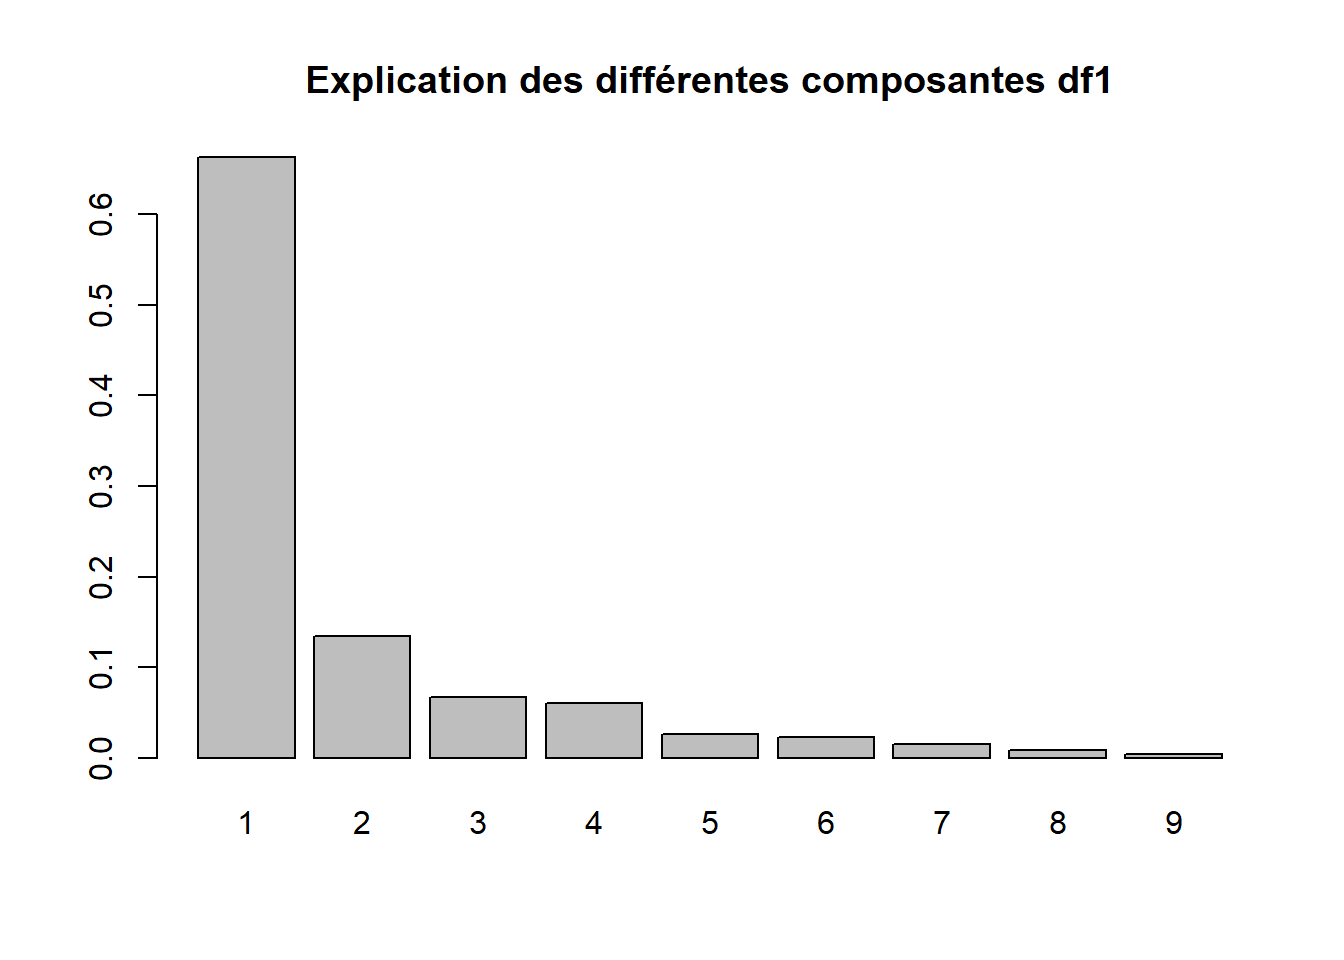
\includegraphics{seshat_laurent_files/figure-latex/unnamed-chunk-4-1.pdf}

\begin{Shaded}
\begin{Highlighting}[]
\KeywordTok{barplot}\NormalTok{(lambda2}\OperatorTok{/}\KeywordTok{sum}\NormalTok{(lambda2),}\DataTypeTok{names.arg =} \DecValTok{1}\OperatorTok{:}\KeywordTok{length}\NormalTok{(lambda2))}
\KeywordTok{title}\NormalTok{(}\DataTypeTok{main=}\StringTok{"Explication des différentes composantes df2"}\NormalTok{)}
\end{Highlighting}
\end{Shaded}

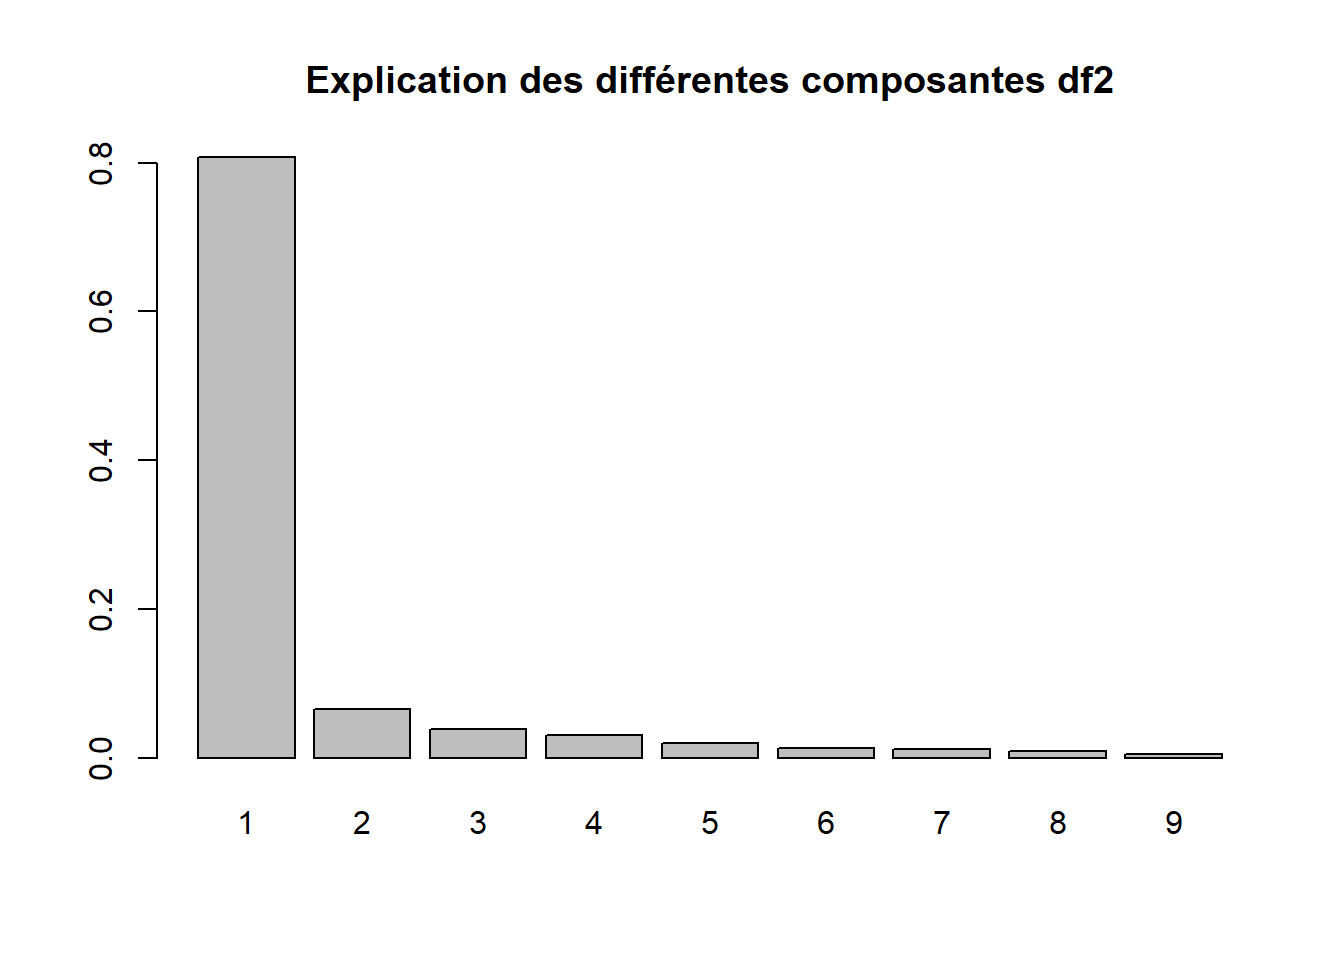
\includegraphics{seshat_laurent_files/figure-latex/unnamed-chunk-4-2.pdf}

\begin{Shaded}
\begin{Highlighting}[]
\KeywordTok{barplot}\NormalTok{(lambda3}\OperatorTok{/}\KeywordTok{sum}\NormalTok{(lambda3),}\DataTypeTok{names.arg =} \DecValTok{1}\OperatorTok{:}\KeywordTok{length}\NormalTok{(lambda3))}
\KeywordTok{title}\NormalTok{(}\DataTypeTok{main=}\StringTok{"Explication des différentes composantes df3"}\NormalTok{)}
\end{Highlighting}
\end{Shaded}

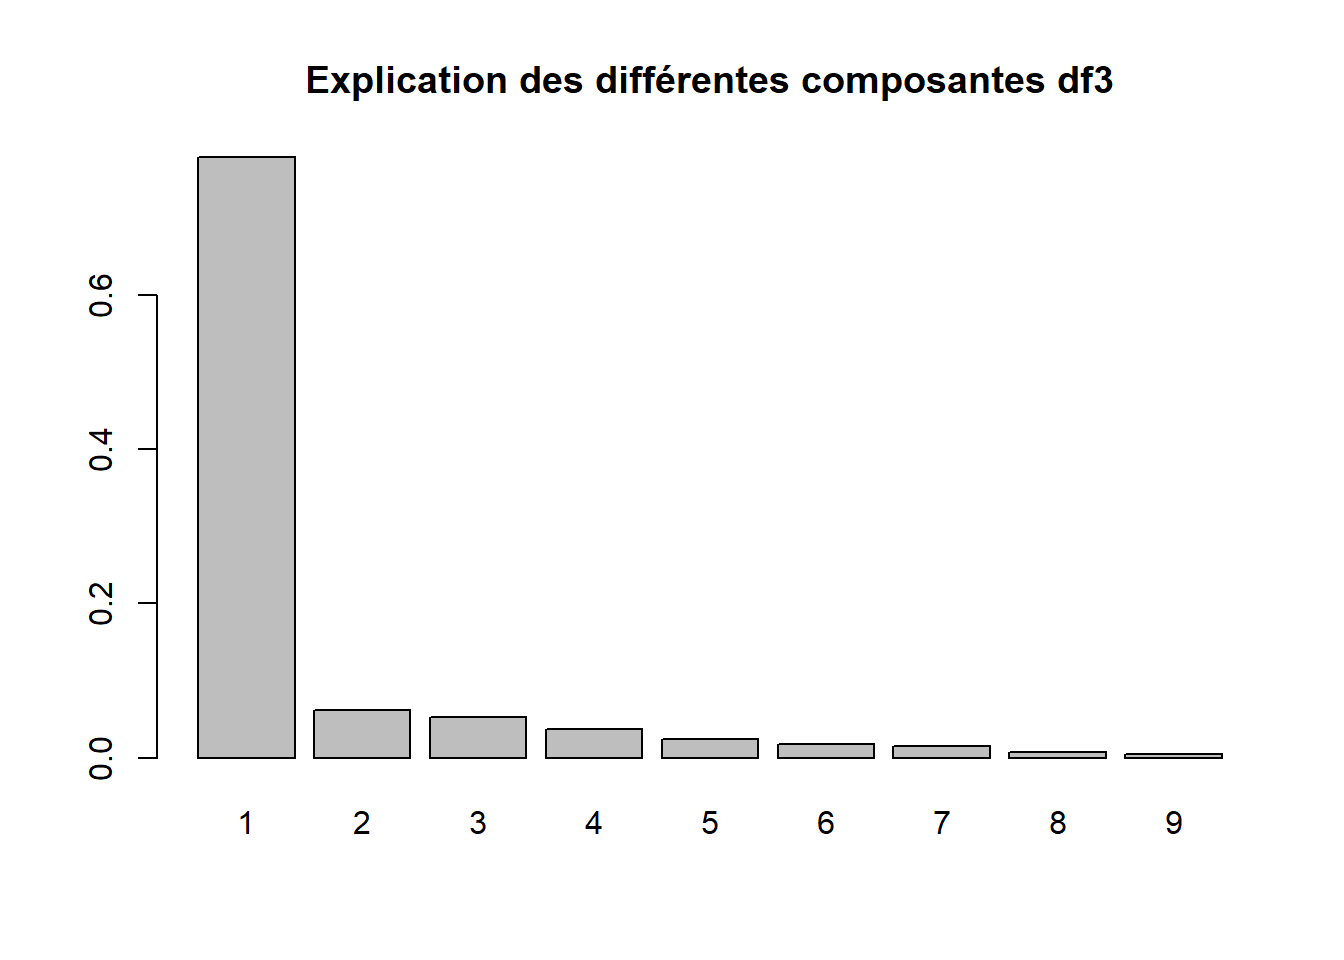
\includegraphics{seshat_laurent_files/figure-latex/unnamed-chunk-4-3.pdf}

\begin{Shaded}
\begin{Highlighting}[]
\CommentTok{# Les composantes principales : }
\NormalTok{C1 =}\StringTok{ }\NormalTok{X1 }\OperatorTok\StringTok{ }\NormalTok{vecteurs_propres_df1 }\CommentTok{#changement de base vers la nouvelle base des composantes principales}
\NormalTok{C2 =}\StringTok{ }\NormalTok{X2 }\OperatorTok\StringTok{ }\NormalTok{vecteurs_propres_df2}
\NormalTok{C3 =}\StringTok{ }\NormalTok{X3 }\OperatorTok\StringTok{ }\NormalTok{vecteurs_propres_df3}

\CommentTok{##Graphique : projection sur les 2 premiers axes principaux}
\CommentTok{# colnames(C) =   paste("comp", 1:4)}
\KeywordTok{plot}\NormalTok{(C1[,}\DecValTok{1}\OperatorTok{:}\DecValTok{2}\NormalTok{],}\DataTypeTok{type=}\StringTok{"p"}\NormalTok{,}\DataTypeTok{xlab=}\StringTok{'PC1'}\NormalTok{,}\DataTypeTok{ylab=}\StringTok{'PC2'}\NormalTok{)}
\KeywordTok{lines}\NormalTok{(}\KeywordTok{c}\NormalTok{(}\KeywordTok{min}\NormalTok{(C1[,}\DecValTok{1}\NormalTok{]),}\KeywordTok{max}\NormalTok{(C1[,}\DecValTok{1}\NormalTok{])),}\KeywordTok{c}\NormalTok{(}\DecValTok{0}\NormalTok{,}\DecValTok{0}\NormalTok{))}
\KeywordTok{lines}\NormalTok{(}\KeywordTok{c}\NormalTok{(}\DecValTok{0}\NormalTok{,}\DecValTok{0}\NormalTok{),}\KeywordTok{c}\NormalTok{(}\KeywordTok{min}\NormalTok{(C1[,}\DecValTok{2}\NormalTok{]),}\KeywordTok{max}\NormalTok{(C1[,}\DecValTok{2}\NormalTok{])))}
\KeywordTok{title}\NormalTok{(}\DataTypeTok{main=}\StringTok{"Projection sur les 2 premiers axes principaux df1"}\NormalTok{)}
\end{Highlighting}
\end{Shaded}

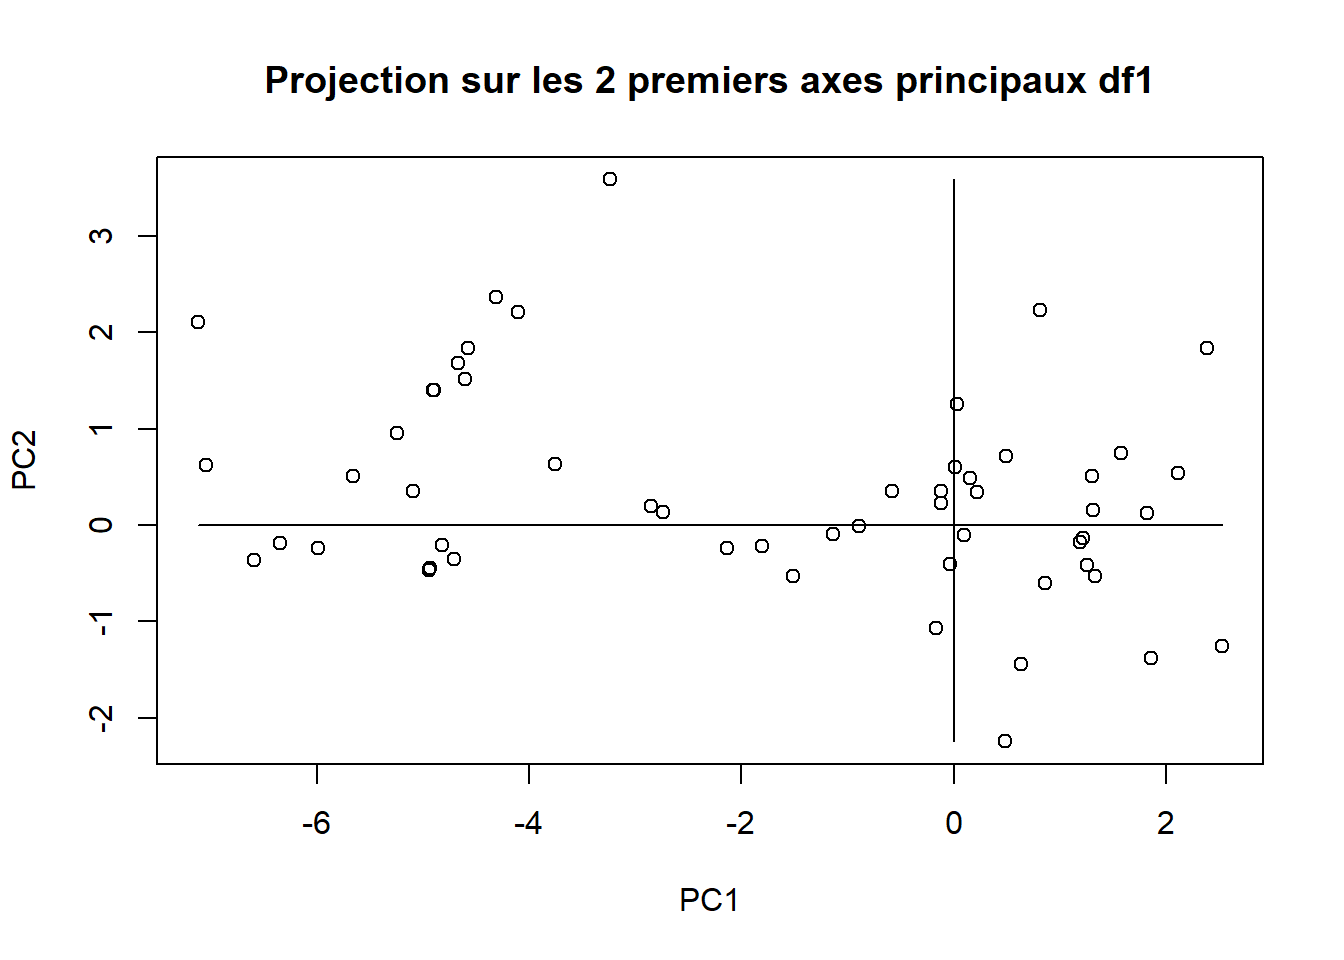
\includegraphics{seshat_laurent_files/figure-latex/unnamed-chunk-4-4.pdf}

\begin{Shaded}
\begin{Highlighting}[]
\KeywordTok{plot}\NormalTok{(C2[,}\DecValTok{1}\OperatorTok{:}\DecValTok{2}\NormalTok{],}\DataTypeTok{type=}\StringTok{"p"}\NormalTok{,}\DataTypeTok{xlab=}\StringTok{'PC1'}\NormalTok{,}\DataTypeTok{ylab=}\StringTok{'PC2'}\NormalTok{)}
\KeywordTok{lines}\NormalTok{(}\KeywordTok{c}\NormalTok{(}\KeywordTok{min}\NormalTok{(C2[,}\DecValTok{1}\NormalTok{]),}\KeywordTok{max}\NormalTok{(C2[,}\DecValTok{1}\NormalTok{])),}\KeywordTok{c}\NormalTok{(}\DecValTok{0}\NormalTok{,}\DecValTok{0}\NormalTok{))}
\KeywordTok{lines}\NormalTok{(}\KeywordTok{c}\NormalTok{(}\DecValTok{0}\NormalTok{,}\DecValTok{0}\NormalTok{),}\KeywordTok{c}\NormalTok{(}\KeywordTok{min}\NormalTok{(C2[,}\DecValTok{2}\NormalTok{]),}\KeywordTok{max}\NormalTok{(C2[,}\DecValTok{2}\NormalTok{])))}
\KeywordTok{title}\NormalTok{(}\DataTypeTok{main=}\StringTok{"Projection sur les 2 premiers axes principaux df2"}\NormalTok{)}
\end{Highlighting}
\end{Shaded}

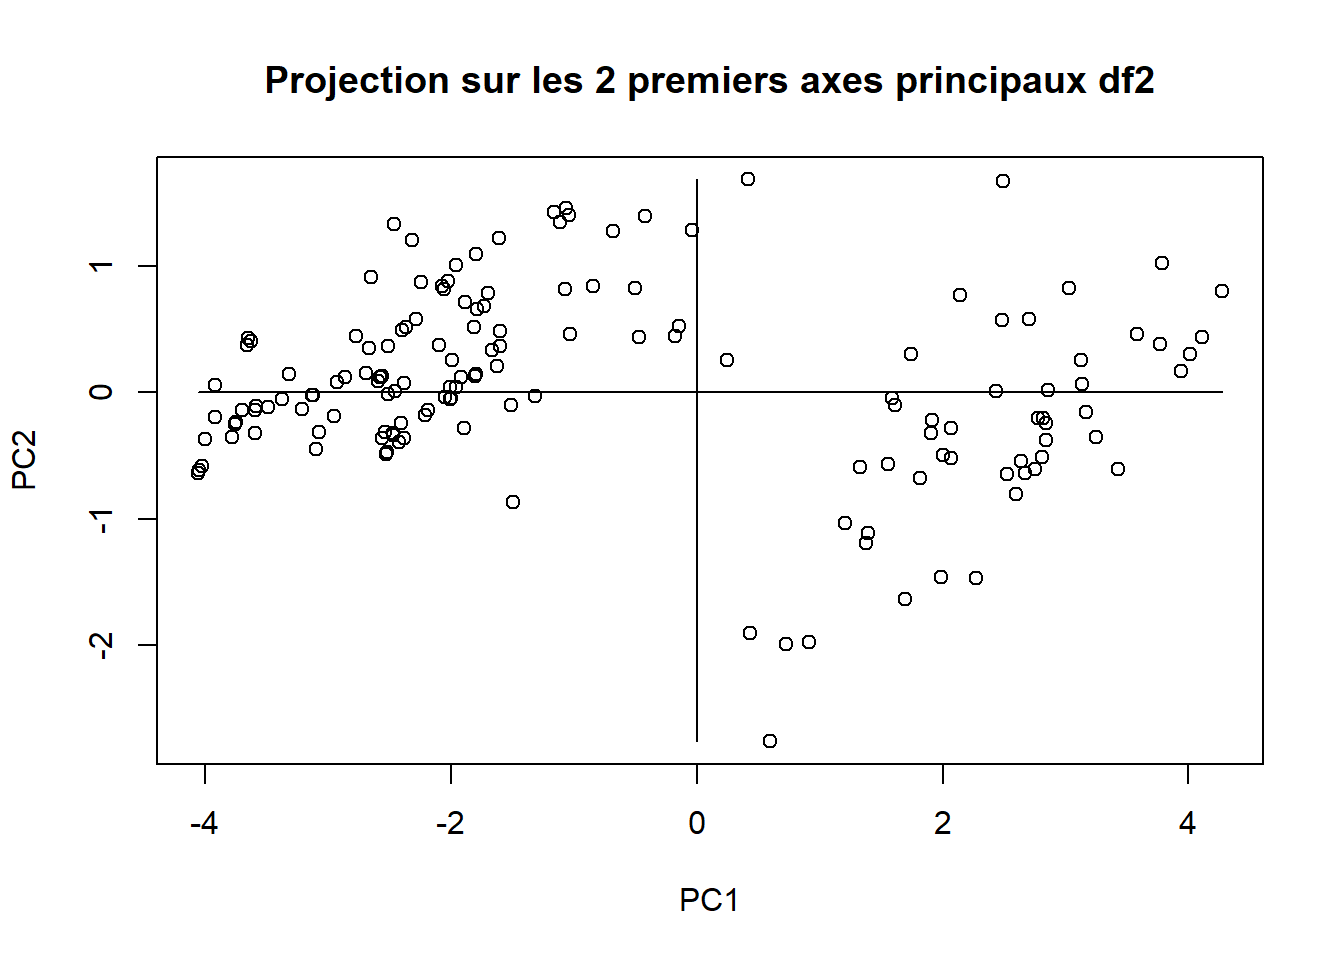
\includegraphics{seshat_laurent_files/figure-latex/unnamed-chunk-4-5.pdf}

\begin{Shaded}
\begin{Highlighting}[]
\KeywordTok{plot}\NormalTok{(C3[,}\DecValTok{1}\OperatorTok{:}\DecValTok{2}\NormalTok{],}\DataTypeTok{type=}\StringTok{"p"}\NormalTok{,}\DataTypeTok{xlab=}\StringTok{'PC1'}\NormalTok{,}\DataTypeTok{ylab=}\StringTok{'PC2'}\NormalTok{)}
\KeywordTok{lines}\NormalTok{(}\KeywordTok{c}\NormalTok{(}\KeywordTok{min}\NormalTok{(C3[,}\DecValTok{1}\NormalTok{]),}\KeywordTok{max}\NormalTok{(C3[,}\DecValTok{1}\NormalTok{])),}\KeywordTok{c}\NormalTok{(}\DecValTok{0}\NormalTok{,}\DecValTok{0}\NormalTok{))}
\KeywordTok{lines}\NormalTok{(}\KeywordTok{c}\NormalTok{(}\DecValTok{0}\NormalTok{,}\DecValTok{0}\NormalTok{),}\KeywordTok{c}\NormalTok{(}\KeywordTok{min}\NormalTok{(C3[,}\DecValTok{2}\NormalTok{]),}\KeywordTok{max}\NormalTok{(C3[,}\DecValTok{2}\NormalTok{])))}
\KeywordTok{title}\NormalTok{(}\DataTypeTok{main=}\StringTok{"Projection sur les 2 premiers axes principaux df3"}\NormalTok{)}
\end{Highlighting}
\end{Shaded}

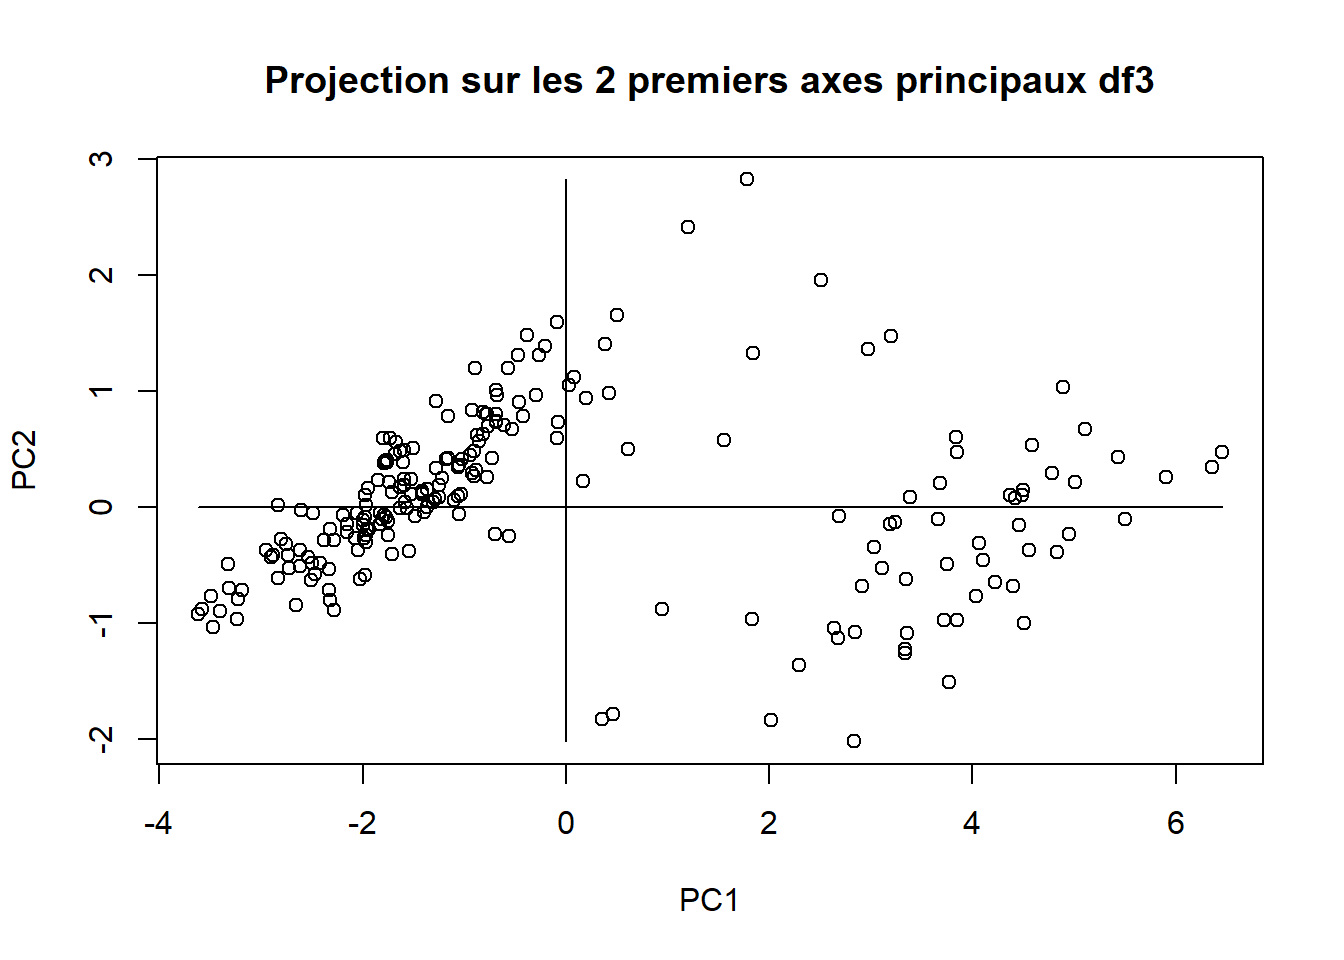
\includegraphics{seshat_laurent_files/figure-latex/unnamed-chunk-4-6.pdf}

\begin{Shaded}
\begin{Highlighting}[]
\CommentTok{# str(C)}
\CommentTok{# text(C[,1:2])}

\CommentTok{## Graphique : contributions des variables au PC1}
\KeywordTok{barplot}\NormalTok{(}\OperatorTok{-}\NormalTok{vecteurs_propres_df1[,}\DecValTok{1}\NormalTok{],}\DataTypeTok{ylab =} \StringTok{'Contribution'}\NormalTok{,}\DataTypeTok{xlab =} \StringTok{'Variables'}\NormalTok{,}\DataTypeTok{names.arg =} \KeywordTok{names}\NormalTok{(df1),}\DataTypeTok{axes =} \OtherTok{TRUE}\NormalTok{)}
\KeywordTok{title}\NormalTok{(}\DataTypeTok{main=}\StringTok{"Contributions des variables au PC1 (df1)"}\NormalTok{)}
\end{Highlighting}
\end{Shaded}

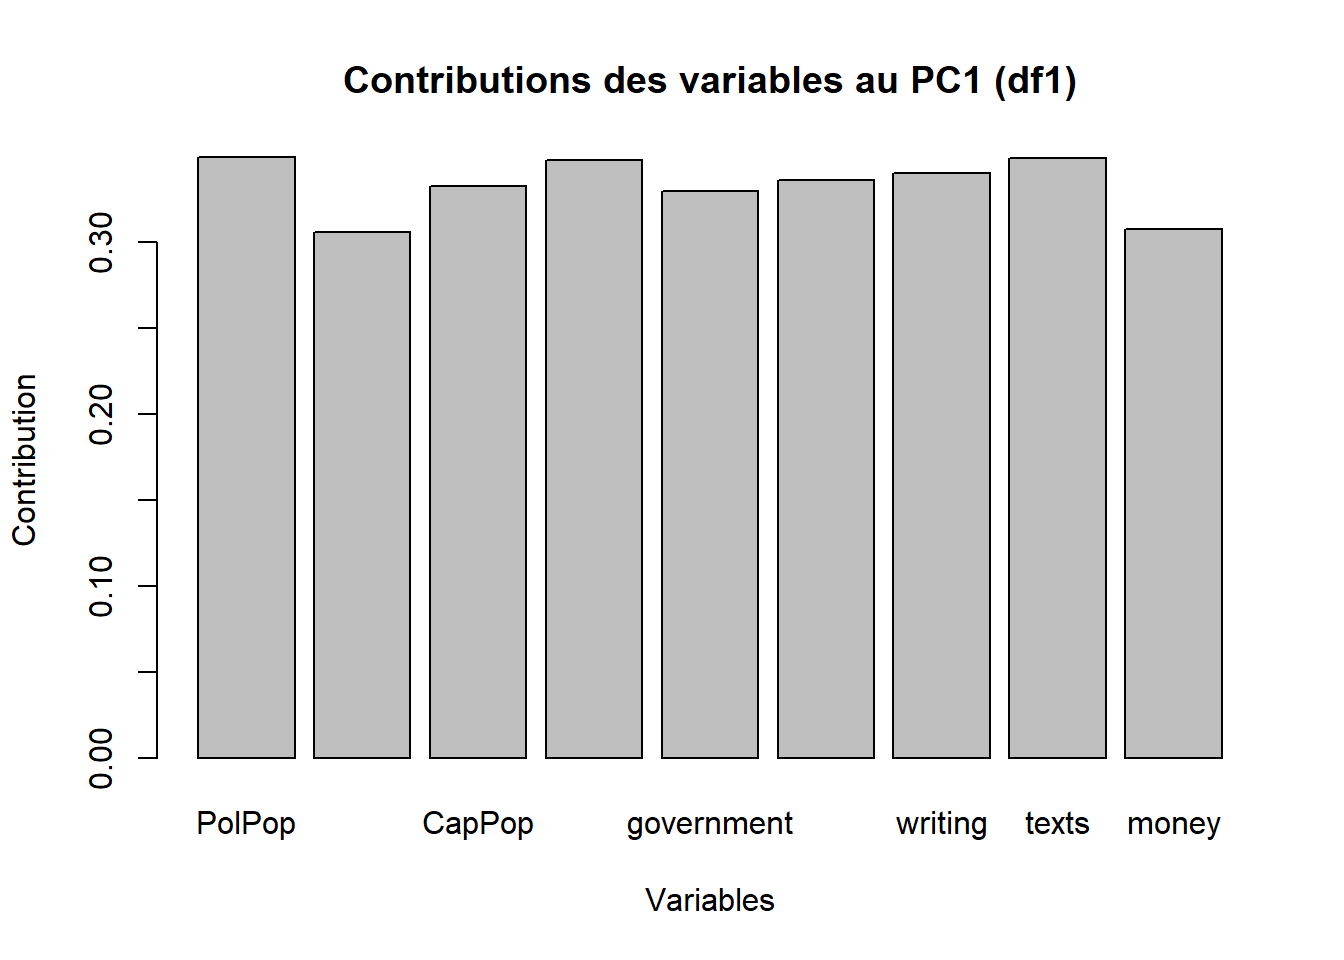
\includegraphics{seshat_laurent_files/figure-latex/unnamed-chunk-4-7.pdf}

\begin{Shaded}
\begin{Highlighting}[]
\KeywordTok{barplot}\NormalTok{(}\OperatorTok{-}\NormalTok{vecteurs_propres_df2[,}\DecValTok{1}\NormalTok{],}\DataTypeTok{ylab =} \StringTok{'Contribution'}\NormalTok{,}\DataTypeTok{xlab =} \StringTok{'Variables'}\NormalTok{,}\DataTypeTok{names.arg =} \KeywordTok{names}\NormalTok{(df2),}\DataTypeTok{axes =} \OtherTok{TRUE}\NormalTok{)}
\KeywordTok{title}\NormalTok{(}\DataTypeTok{main=}\StringTok{"Contributions des variables au PC1 (df2)"}\NormalTok{)}
\end{Highlighting}
\end{Shaded}

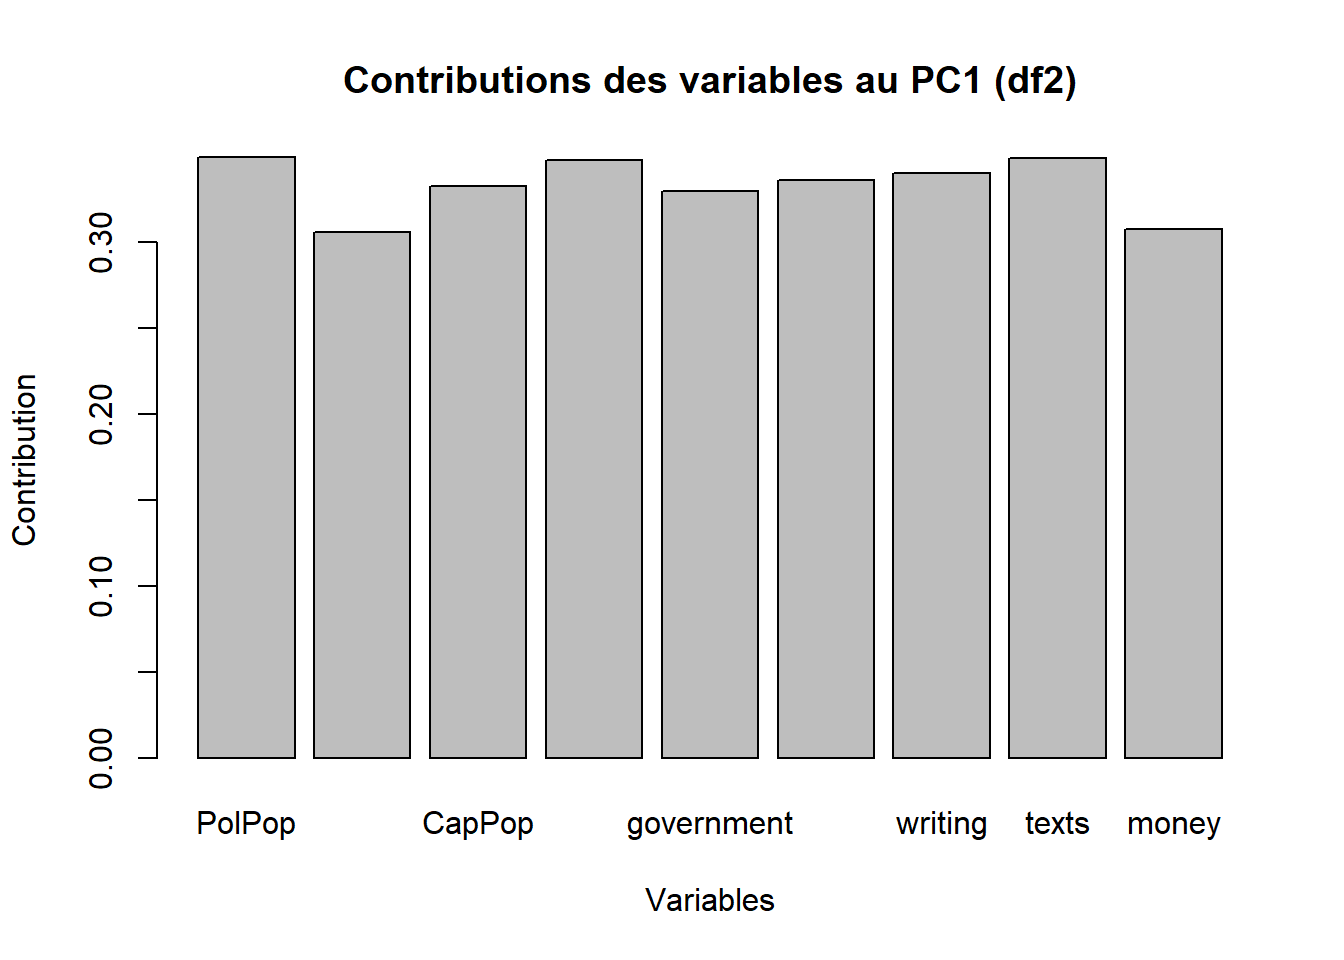
\includegraphics{seshat_laurent_files/figure-latex/unnamed-chunk-4-8.pdf}

\begin{Shaded}
\begin{Highlighting}[]
\KeywordTok{barplot}\NormalTok{(}\OperatorTok{-}\NormalTok{vecteurs_propres_df3[,}\DecValTok{1}\NormalTok{],}\DataTypeTok{ylab =} \StringTok{'Contribution'}\NormalTok{,}\DataTypeTok{xlab =} \StringTok{'Variables'}\NormalTok{,}\DataTypeTok{names.arg =} \KeywordTok{names}\NormalTok{(df3),}\DataTypeTok{axes =} \OtherTok{TRUE}\NormalTok{)}
\KeywordTok{title}\NormalTok{(}\DataTypeTok{main=}\StringTok{"Contributions des variables au PC1 (df3)"}\NormalTok{)}
\end{Highlighting}
\end{Shaded}

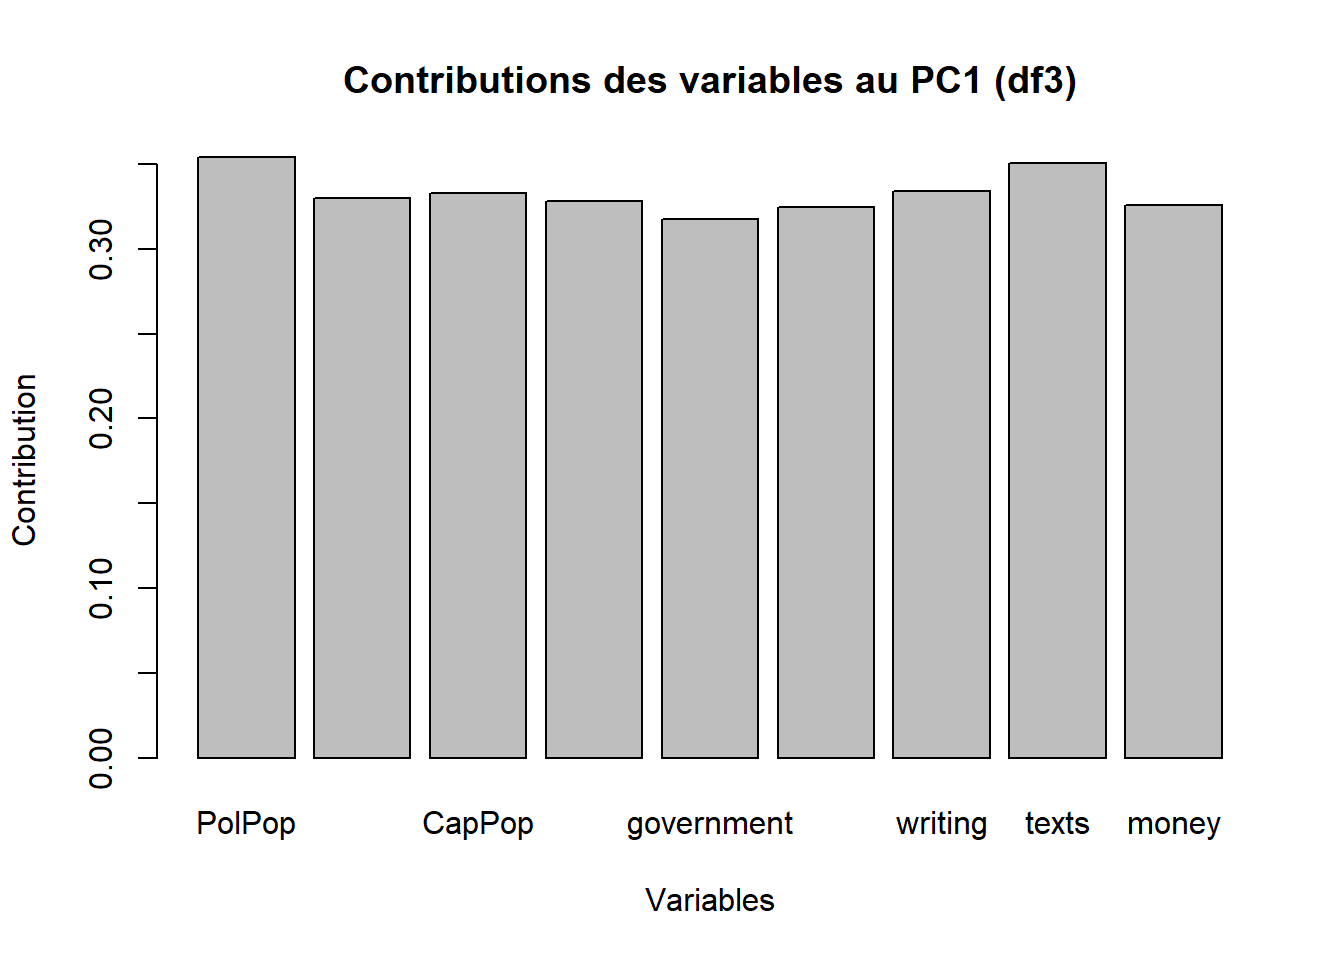
\includegraphics{seshat_laurent_files/figure-latex/unnamed-chunk-4-9.pdf}

\begin{Shaded}
\begin{Highlighting}[]
\CommentTok{## Graphique : contributions des variables au PC2}
\KeywordTok{barplot}\NormalTok{(}\OperatorTok{-}\NormalTok{vecteurs_propres_df1[,}\DecValTok{2}\NormalTok{],}\DataTypeTok{ylab =} \StringTok{'Contribution'}\NormalTok{,}\DataTypeTok{xlab =} \StringTok{'Variables'}\NormalTok{,}\DataTypeTok{names.arg =} \KeywordTok{names}\NormalTok{(df1),}\DataTypeTok{axes =} \OtherTok{TRUE}\NormalTok{)}
\KeywordTok{title}\NormalTok{(}\DataTypeTok{main=}\StringTok{"Contributions des variables au PC2 (df1)"}\NormalTok{)}
\end{Highlighting}
\end{Shaded}

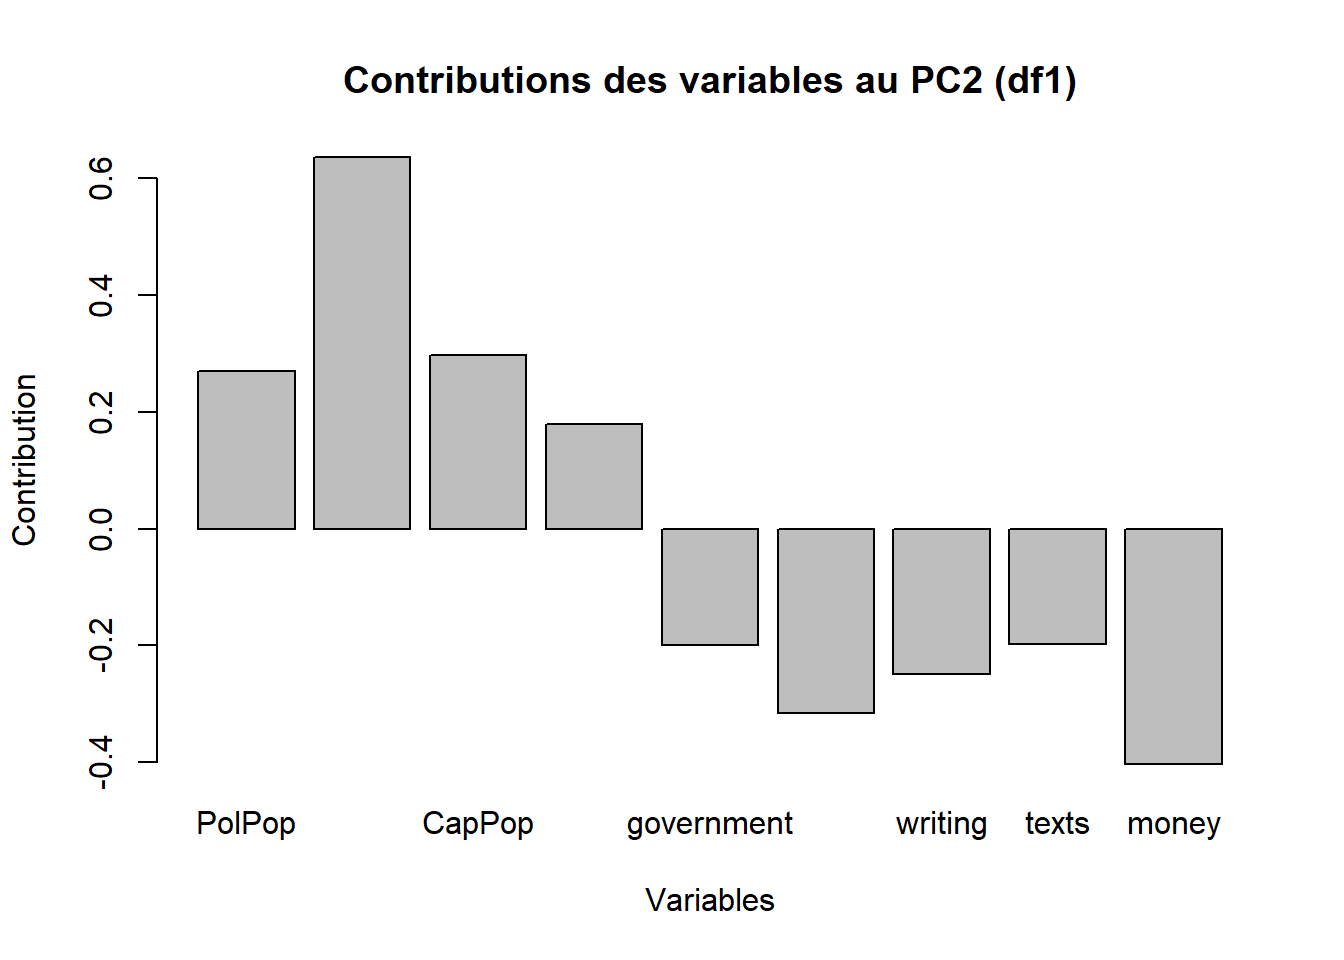
\includegraphics{seshat_laurent_files/figure-latex/unnamed-chunk-4-10.pdf}

\begin{Shaded}
\begin{Highlighting}[]
\KeywordTok{barplot}\NormalTok{(}\OperatorTok{-}\NormalTok{vecteurs_propres_df2[,}\DecValTok{2}\NormalTok{],}\DataTypeTok{ylab =} \StringTok{'Contribution'}\NormalTok{,}\DataTypeTok{xlab =} \StringTok{'Variables'}\NormalTok{,}\DataTypeTok{names.arg =} \KeywordTok{names}\NormalTok{(df2),}\DataTypeTok{axes =} \OtherTok{TRUE}\NormalTok{)}
\KeywordTok{title}\NormalTok{(}\DataTypeTok{main=}\StringTok{"Contributions des variables au PC2 (df2)"}\NormalTok{)}
\end{Highlighting}
\end{Shaded}

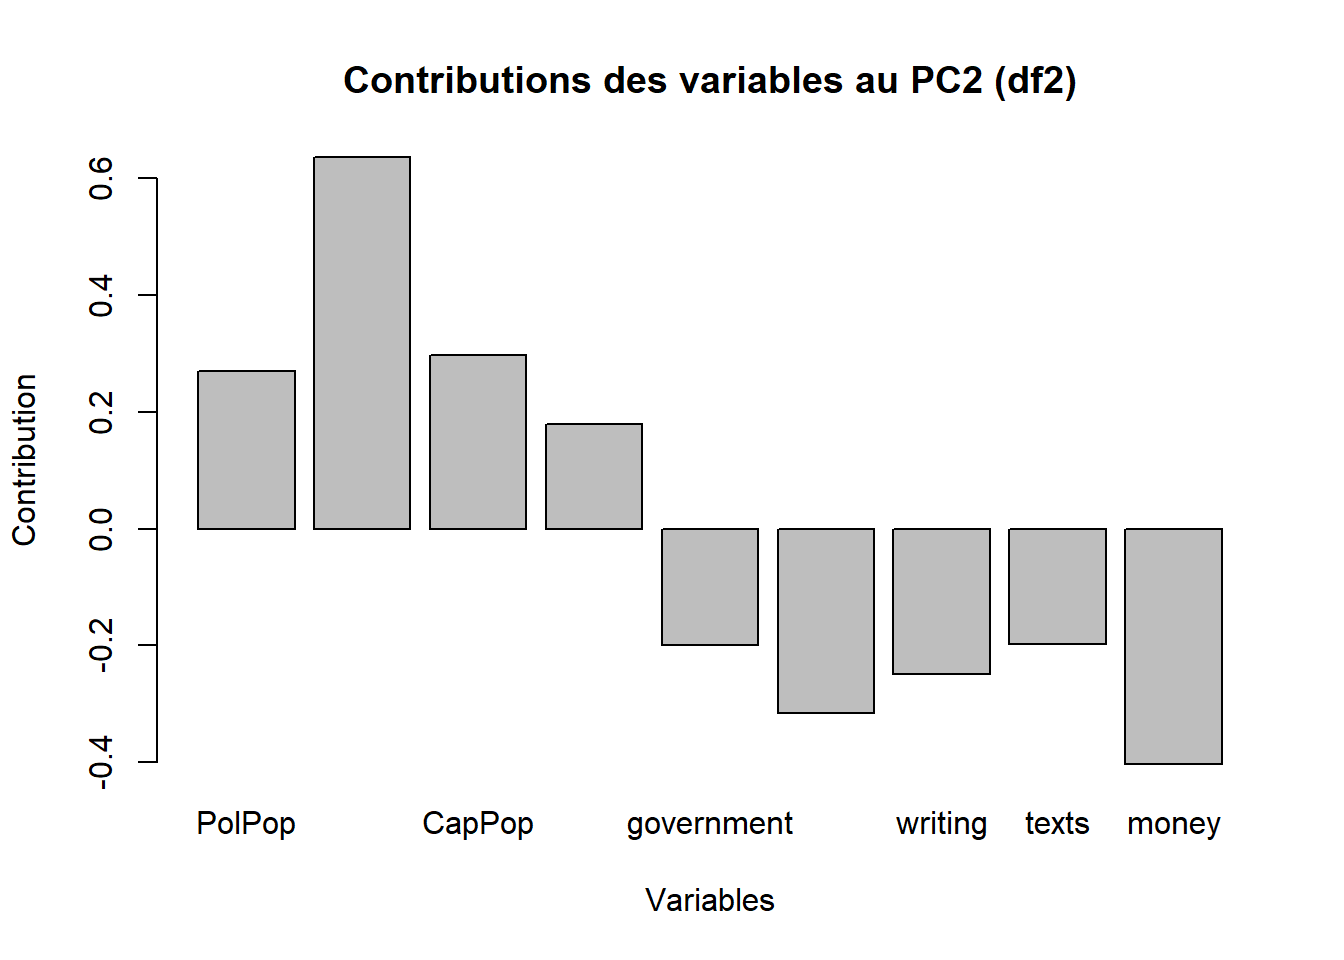
\includegraphics{seshat_laurent_files/figure-latex/unnamed-chunk-4-11.pdf}

\begin{Shaded}
\begin{Highlighting}[]
\KeywordTok{barplot}\NormalTok{(}\OperatorTok{-}\NormalTok{vecteurs_propres_df3[,}\DecValTok{2}\NormalTok{],}\DataTypeTok{ylab =} \StringTok{'Contribution'}\NormalTok{,}\DataTypeTok{xlab =} \StringTok{'Variables'}\NormalTok{,}\DataTypeTok{names.arg =} \KeywordTok{names}\NormalTok{(df3),}\DataTypeTok{axes =} \OtherTok{TRUE}\NormalTok{)}
\KeywordTok{title}\NormalTok{(}\DataTypeTok{main=}\StringTok{"Contributions des variables au PC2 (df3)"}\NormalTok{)}
\end{Highlighting}
\end{Shaded}

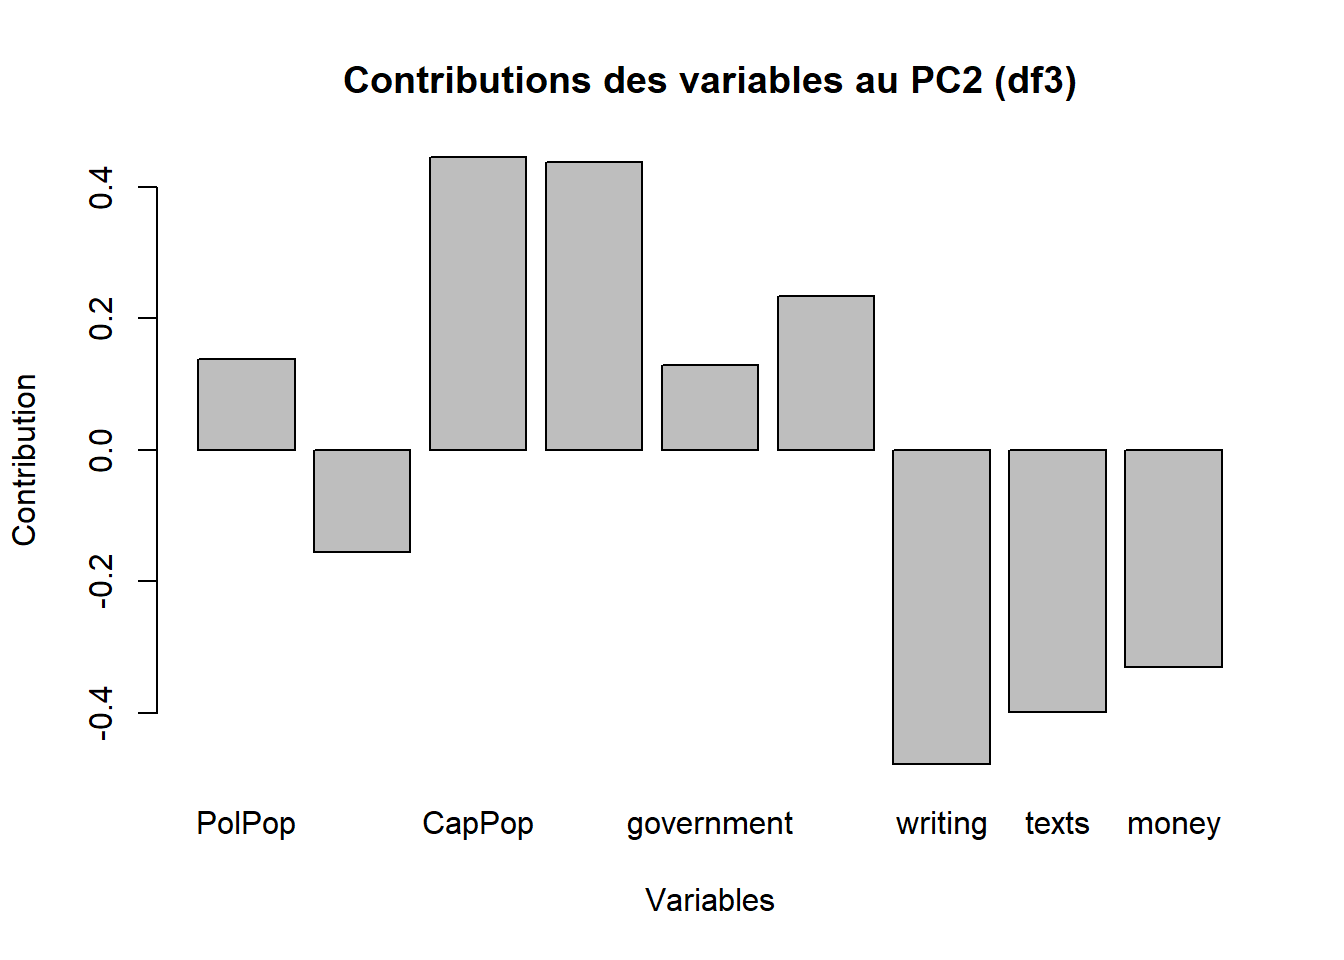
\includegraphics{seshat_laurent_files/figure-latex/unnamed-chunk-4-12.pdf}

Remarquer que : * La premiere composante explique tout : interpréter *
On peut remarquer deux clusters sur l'ACP pour df2 et df3, et vaguement
pour df1. * Toutes les variables contribuent de la même façon au PC1,
interpréter * Pour le pc2 on observe des nuances d'ordre similaire, voir
cercle

\begin{Shaded}
\begin{Highlighting}[]
\KeywordTok{library}\NormalTok{(FactoMineR)}
\NormalTok{pca1 <-}\StringTok{ }\KeywordTok{PCA}\NormalTok{(df1, }\DataTypeTok{scale.unit =} \OtherTok{TRUE}\NormalTok{, }\DataTypeTok{ncp =} \DecValTok{11}\NormalTok{, }\DataTypeTok{graph =} \OtherTok{TRUE}\NormalTok{)}
\end{Highlighting}
\end{Shaded}

\includegraphics{seshat_laurent_files/figure-latex/unnamed-chunk-5-1.pdf}
\includegraphics{seshat_laurent_files/figure-latex/unnamed-chunk-5-2.pdf}

\begin{Shaded}
\begin{Highlighting}[]
\NormalTok{pca2 <-}\StringTok{ }\KeywordTok{PCA}\NormalTok{(df2, }\DataTypeTok{scale.unit =} \OtherTok{TRUE}\NormalTok{, }\DataTypeTok{ncp =} \DecValTok{11}\NormalTok{, }\DataTypeTok{graph =} \OtherTok{TRUE}\NormalTok{)}
\end{Highlighting}
\end{Shaded}

\includegraphics{seshat_laurent_files/figure-latex/unnamed-chunk-5-3.pdf}
\includegraphics{seshat_laurent_files/figure-latex/unnamed-chunk-5-4.pdf}

\begin{Shaded}
\begin{Highlighting}[]
\NormalTok{pca3 <-}\StringTok{ }\KeywordTok{PCA}\NormalTok{(df3, }\DataTypeTok{scale.unit =} \OtherTok{TRUE}\NormalTok{, }\DataTypeTok{ncp =} \DecValTok{11}\NormalTok{, }\DataTypeTok{graph =} \OtherTok{TRUE}\NormalTok{)}
\end{Highlighting}
\end{Shaded}

\includegraphics{seshat_laurent_files/figure-latex/unnamed-chunk-5-5.pdf}
\includegraphics{seshat_laurent_files/figure-latex/unnamed-chunk-5-6.pdf}

\begin{Shaded}
\begin{Highlighting}[]
\NormalTok{pca1}\OperatorTok{$}\NormalTok{var}\OperatorTok{$}\NormalTok{cos2}
\end{Highlighting}
\end{Shaded}

\begin{verbatim}
##                Dim.1        Dim.2       Dim.3      Dim.4       Dim.5
## PolPop     0.5480879 0.1862429827 0.044610416 0.13352522 0.024185491
## PolTerr    0.2919821 0.6082472800 0.001446941 0.00787346 0.032036155
## CapPop     0.6120063 0.0799277063 0.211792702 0.04149435 0.025010495
## levels     0.7857457 0.0001943283 0.128514947 0.01235059 0.001207864
## government 0.8113615 0.0022837852 0.030996229 0.01687948 0.091604837
## infrastr   0.8193441 0.0848232482 0.002981826 0.01051048 0.010045029
## writing    0.8244034 0.0087005542 0.072980851 0.04093629 0.003896583
## texts      0.8141004 0.0004716739 0.083586406 0.04168255 0.017766575
## money      0.4632368 0.2346856126 0.021351194 0.23728771 0.027034827
##                   Dim.6        Dim.7        Dim.8        Dim.9
## PolPop     0.0588487532 3.450635e-03 1.042695e-03 5.954671e-06
## PolTerr    0.0573465790 1.008333e-03 8.498845e-07 5.825597e-05
## CapPop     0.0001469855 1.805757e-02 1.084856e-02 7.152979e-04
## levels     0.0015140486 5.811496e-02 1.046142e-02 1.896143e-03
## government 0.0280080096 8.969107e-05 1.831439e-02 4.620572e-04
## infrastr   0.0098475873 2.757510e-02 3.316902e-02 1.703558e-03
## writing    0.0225040149 1.161241e-02 6.833932e-05 1.489761e-02
## texts      0.0218555495 6.141516e-03 6.350979e-04 1.376024e-02
## money      0.0026813741 9.612215e-03 3.984873e-03 1.254030e-04
\end{verbatim}

\begin{Shaded}
\begin{Highlighting}[]
\NormalTok{pca2}\OperatorTok{$}\NormalTok{var}\OperatorTok{$}\NormalTok{cos2}
\end{Highlighting}
\end{Shaded}

\begin{verbatim}
##                Dim.1      Dim.2        Dim.3        Dim.4        Dim.5
## PolPop     0.8866682 0.04314752 4.557820e-04 1.375375e-02 0.0013488258
## PolTerr    0.6779412 0.23950930 7.964413e-05 4.630314e-02 0.0123025761
## CapPop     0.8030639 0.05203719 2.983147e-03 6.445691e-02 0.0491928179
## levels     0.8777989 0.01887088 2.068383e-02 2.658481e-04 0.0031857644
## government 0.7886151 0.02360785 1.034885e-01 4.430183e-03 0.0532406867
## infrastr   0.8209131 0.05877893 1.177569e-02 4.441829e-02 0.0003383528
## writing    0.8401705 0.03672265 5.903167e-03 7.319678e-02 0.0181872672
## texts      0.8848711 0.02315803 7.097974e-03 3.313908e-02 0.0236277329
## money      0.6877348 0.09586542 1.913240e-01 6.882813e-05 0.0145221287
##                   Dim.6        Dim.7        Dim.8        Dim.9
## PolPop     0.0049203182 0.0042585011 0.0383506991 7.096389e-03
## PolTerr    0.0099650093 0.0038802748 0.0086250995 1.393763e-03
## CapPop     0.0170247110 0.0062331741 0.0036915241 1.316628e-03
## levels     0.0057533202 0.0729659756 0.0004222713 5.317289e-05
## government 0.0236382545 0.0017937330 0.0011758575 9.820141e-06
## infrastr   0.0559485326 0.0025864972 0.0025459350 2.694647e-03
## writing    0.0011305446 0.0004000535 0.0136318159 1.065721e-02
## texts      0.0000458897 0.0005421247 0.0081742632 1.934384e-02
## money      0.0002681732 0.0096888149 0.0004999708 2.781695e-05
\end{verbatim}

\begin{Shaded}
\begin{Highlighting}[]
\NormalTok{pca3}\OperatorTok{$}\NormalTok{var}\OperatorTok{$}\NormalTok{cos2}
\end{Highlighting}
\end{Shaded}

\begin{verbatim}
##                Dim.1       Dim.2        Dim.3        Dim.4        Dim.5
## PolPop     0.8789928 0.010512698 4.861760e-02 0.0036408558 0.0052682710
## PolTerr    0.7627377 0.013264257 1.401938e-01 0.0133884055 0.0046917883
## CapPop     0.7754450 0.109350054 2.654505e-02 0.0035750879 0.0091813685
## levels     0.7544318 0.105955826 2.922575e-03 0.0099314500 0.0889040992
## government 0.7074772 0.009162061 1.301755e-01 0.1026371973 0.0153580842
## infrastr   0.7395846 0.030173592 1.081410e-01 0.0194410218 0.0811649807
## writing    0.7812877 0.125536092 6.512958e-05 0.0381611710 0.0007091162
## texts      0.8626199 0.087508689 5.488563e-03 0.0001755454 0.0015636431
## money      0.7444464 0.060053984 7.799727e-03 0.1379810353 0.0154437699
##                   Dim.6        Dim.7        Dim.8        Dim.9
## PolPop     5.321103e-03 0.0020964753 4.317305e-02 0.0023771875
## PolTerr    4.192839e-02 0.0131204183 9.950416e-03 0.0007248116
## CapPop     2.105842e-02 0.0465252879 8.142437e-03 0.0001773008
## levels     7.961671e-03 0.0297783237 1.032057e-04 0.0000110674
## government 2.885371e-02 0.0060569460 5.254681e-05 0.0002267390
## infrastr   3.990936e-06 0.0193004033 3.768058e-05 0.0021527278
## writing    3.778117e-02 0.0007516994 4.301514e-03 0.0114063588
## texts      1.180934e-02 0.0009628496 3.004440e-03 0.0268669925
## money      9.984368e-03 0.0206947210 9.998878e-04 0.0025961013
\end{verbatim}

\begin{Shaded}
\begin{Highlighting}[]
\NormalTok{cos2C1_df1 =}\StringTok{ }\NormalTok{pca1}\OperatorTok{$}\NormalTok{ind}\OperatorTok{$}\NormalTok{cos2[,}\DecValTok{1}\NormalTok{] }\OperatorTok{+}\StringTok{ }\NormalTok{pca1}\OperatorTok{$}\NormalTok{ind}\OperatorTok{$}\NormalTok{cos2[,}\DecValTok{2}\NormalTok{] }\CommentTok{# tous proches de 1 donc  }
\NormalTok{cos2C1_df2 =}\StringTok{ }\NormalTok{pca2}\OperatorTok{$}\NormalTok{ind}\OperatorTok{$}\NormalTok{cos2[,}\DecValTok{1}\NormalTok{] }\OperatorTok{+}\StringTok{ }\NormalTok{pca2}\OperatorTok{$}\NormalTok{ind}\OperatorTok{$}\NormalTok{cos2[,}\DecValTok{2}\NormalTok{] }\CommentTok{# tous proches de 1 donc  }
\NormalTok{cos2C1_df3 =}\StringTok{ }\NormalTok{pca3}\OperatorTok{$}\NormalTok{ind}\OperatorTok{$}\NormalTok{cos2[,}\DecValTok{1}\NormalTok{] }\OperatorTok{+}\StringTok{ }\NormalTok{pca3}\OperatorTok{$}\NormalTok{ind}\OperatorTok{$}\NormalTok{cos2[,}\DecValTok{2}\NormalTok{] }\CommentTok{# tous proches de 1 donc  }
\KeywordTok{length}\NormalTok{(cos2C1_df1[cos2C1_df1 }\OperatorTok{>}\StringTok{ }\FloatTok{0.8}\NormalTok{])}
\end{Highlighting}
\end{Shaded}

\begin{verbatim}
## [1] 111
\end{verbatim}

\begin{Shaded}
\begin{Highlighting}[]
\KeywordTok{length}\NormalTok{(cos2C1_df1[cos2C1_df2 }\OperatorTok{>}\StringTok{ }\FloatTok{0.8}\NormalTok{])}
\end{Highlighting}
\end{Shaded}

\begin{verbatim}
## [1] 207
\end{verbatim}

\begin{Shaded}
\begin{Highlighting}[]
\KeywordTok{length}\NormalTok{(cos2C1_df1[cos2C1_df3 }\OperatorTok{>}\StringTok{ }\FloatTok{0.8}\NormalTok{])}
\end{Highlighting}
\end{Shaded}

\begin{verbatim}
## [1] 159
\end{verbatim}

\begin{Shaded}
\begin{Highlighting}[]
\KeywordTok{plot}\NormalTok{(pca1,}\DataTypeTok{choix=}\StringTok{"ind"}\NormalTok{)    }\CommentTok{# graphe des individus}
\end{Highlighting}
\end{Shaded}

\includegraphics{seshat_laurent_files/figure-latex/unnamed-chunk-5-7.pdf}

\begin{Shaded}
\begin{Highlighting}[]
\KeywordTok{plot}\NormalTok{(pca1,}\DataTypeTok{choix=}\StringTok{"var"}\NormalTok{)    }\CommentTok{# graphe des variables }
\end{Highlighting}
\end{Shaded}

\includegraphics{seshat_laurent_files/figure-latex/unnamed-chunk-5-8.pdf}

\begin{Shaded}
\begin{Highlighting}[]
\KeywordTok{plot}\NormalTok{(pca2,}\DataTypeTok{choix=}\StringTok{"ind"}\NormalTok{)    }\CommentTok{# graphe des individus}
\end{Highlighting}
\end{Shaded}

\includegraphics{seshat_laurent_files/figure-latex/unnamed-chunk-5-9.pdf}

\begin{Shaded}
\begin{Highlighting}[]
\KeywordTok{plot}\NormalTok{(pca2,}\DataTypeTok{choix=}\StringTok{"var"}\NormalTok{)    }\CommentTok{# graphe des variables }
\end{Highlighting}
\end{Shaded}

\includegraphics{seshat_laurent_files/figure-latex/unnamed-chunk-5-10.pdf}

\begin{Shaded}
\begin{Highlighting}[]
\KeywordTok{plot}\NormalTok{(pca3,}\DataTypeTok{choix=}\StringTok{"ind"}\NormalTok{)    }\CommentTok{# graphe des individus}
\end{Highlighting}
\end{Shaded}

\includegraphics{seshat_laurent_files/figure-latex/unnamed-chunk-5-11.pdf}

\begin{Shaded}
\begin{Highlighting}[]
\KeywordTok{plot}\NormalTok{(pca3,}\DataTypeTok{choix=}\StringTok{"var"}\NormalTok{)    }\CommentTok{# graphe des variables }
\end{Highlighting}
\end{Shaded}

\includegraphics{seshat_laurent_files/figure-latex/unnamed-chunk-5-12.pdf}

\begin{Shaded}
\begin{Highlighting}[]
\KeywordTok{plot}\NormalTok{(pca1, }\DataTypeTok{cex=}\NormalTok{pca1}\OperatorTok{$}\NormalTok{ind}\OperatorTok{$}\NormalTok{cos2, }\DataTypeTok{choix=}\StringTok{"ind"}\NormalTok{)}
\end{Highlighting}
\end{Shaded}

\begin{verbatim}
## Warning in ggoptions["size"] <- 4 * argument$cex: le nombre d'objets à remplacer
## n'est pas multiple de la taille du remplacement
\end{verbatim}

\includegraphics{seshat_laurent_files/figure-latex/unnamed-chunk-5-13.pdf}

\begin{Shaded}
\begin{Highlighting}[]
\KeywordTok{plot}\NormalTok{(pca2, }\DataTypeTok{cex=}\NormalTok{pca2}\OperatorTok{$}\NormalTok{ind}\OperatorTok{$}\NormalTok{cos2, }\DataTypeTok{choix=}\StringTok{"ind"}\NormalTok{)}
\end{Highlighting}
\end{Shaded}

\begin{verbatim}
## Warning in ggoptions["size"] <- 4 * argument$cex: le nombre d'objets à remplacer
## n'est pas multiple de la taille du remplacement
\end{verbatim}

\includegraphics{seshat_laurent_files/figure-latex/unnamed-chunk-5-14.pdf}

\begin{Shaded}
\begin{Highlighting}[]
\KeywordTok{plot}\NormalTok{(pca3, }\DataTypeTok{cex=}\NormalTok{pca3}\OperatorTok{$}\NormalTok{ind}\OperatorTok{$}\NormalTok{cos2, }\DataTypeTok{choix=}\StringTok{"ind"}\NormalTok{)}
\end{Highlighting}
\end{Shaded}

\begin{verbatim}
## Warning in ggoptions["size"] <- 4 * argument$cex: le nombre d'objets à remplacer
## n'est pas multiple de la taille du remplacement
\end{verbatim}

\includegraphics{seshat_laurent_files/figure-latex/unnamed-chunk-5-15.pdf}

\begin{Shaded}
\begin{Highlighting}[]
\KeywordTok{plot}\NormalTok{(pca1, }\DataTypeTok{select=}\StringTok{"cos2 0.8"}\NormalTok{, }\DataTypeTok{choix=}\StringTok{"ind"}\NormalTok{)}
\end{Highlighting}
\end{Shaded}

\includegraphics{seshat_laurent_files/figure-latex/unnamed-chunk-5-16.pdf}

\begin{Shaded}
\begin{Highlighting}[]
\KeywordTok{plot}\NormalTok{(pca2, }\DataTypeTok{select=}\StringTok{"cos2 0.8"}\NormalTok{, }\DataTypeTok{choix=}\StringTok{"ind"}\NormalTok{)}
\end{Highlighting}
\end{Shaded}

\includegraphics{seshat_laurent_files/figure-latex/unnamed-chunk-5-17.pdf}

\begin{Shaded}
\begin{Highlighting}[]
\KeywordTok{plot}\NormalTok{(pca3, }\DataTypeTok{select=}\StringTok{"cos2 0.8"}\NormalTok{, }\DataTypeTok{choix=}\StringTok{"ind"}\NormalTok{)}
\end{Highlighting}
\end{Shaded}

\includegraphics{seshat_laurent_files/figure-latex/unnamed-chunk-5-18.pdf}

\hypertarget{k-means-et-cah}{%
\subsubsection{3.3 k-means et CAH}\label{k-means-et-cah}}

On a vu sur l'ACP qu'on pouvait distinguer environ deux groupes. On
essaie des k-means :

\begin{Shaded}
\begin{Highlighting}[]
\NormalTok{kmeans.result =}\StringTok{ }\KeywordTok{kmeans}\NormalTok{(df1,}\DecValTok{3}\NormalTok{)}
\KeywordTok{plot}\NormalTok{(C1[,}\DecValTok{1}\OperatorTok{:}\DecValTok{2}\NormalTok{],}\DataTypeTok{type=}\StringTok{"p"}\NormalTok{,}\DataTypeTok{xlab=}\StringTok{'PC1'}\NormalTok{,}\DataTypeTok{ylab=}\StringTok{'PC2'}\NormalTok{,}\DataTypeTok{col =}\NormalTok{ kmeans.result}\OperatorTok{$}\NormalTok{cluster}\OperatorTok{+}\DecValTok{3}\NormalTok{, }\DataTypeTok{main=}\StringTok{"df1, k = 3"}\NormalTok{)}
\end{Highlighting}
\end{Shaded}

\includegraphics{seshat_laurent_files/figure-latex/unnamed-chunk-6-1.pdf}

\begin{Shaded}
\begin{Highlighting}[]
\NormalTok{kmeans.result =}\StringTok{ }\KeywordTok{kmeans}\NormalTok{(df1,}\DecValTok{2}\NormalTok{)}
\KeywordTok{plot}\NormalTok{(C1[,}\DecValTok{1}\OperatorTok{:}\DecValTok{2}\NormalTok{],}\DataTypeTok{type=}\StringTok{"p"}\NormalTok{,}\DataTypeTok{xlab=}\StringTok{'PC1'}\NormalTok{,}\DataTypeTok{ylab=}\StringTok{'PC2'}\NormalTok{,}\DataTypeTok{col =}\NormalTok{ kmeans.result}\OperatorTok{$}\NormalTok{cluster, }\DataTypeTok{main=}\StringTok{"df1, k = 2"}\NormalTok{)}
\end{Highlighting}
\end{Shaded}

\includegraphics{seshat_laurent_files/figure-latex/unnamed-chunk-6-2.pdf}

\begin{Shaded}
\begin{Highlighting}[]
\NormalTok{kmeans.result =}\StringTok{ }\KeywordTok{kmeans}\NormalTok{(df2,}\DecValTok{2}\NormalTok{)}
\KeywordTok{plot}\NormalTok{(C2[,}\DecValTok{1}\OperatorTok{:}\DecValTok{2}\NormalTok{],}\DataTypeTok{type=}\StringTok{"p"}\NormalTok{,}\DataTypeTok{xlab=}\StringTok{'PC1'}\NormalTok{,}\DataTypeTok{ylab=}\StringTok{'PC2'}\NormalTok{,}\DataTypeTok{col =}\NormalTok{ kmeans.result}\OperatorTok{$}\NormalTok{cluster, }\DataTypeTok{main=}\StringTok{"df2, k = 2"}\NormalTok{)}
\end{Highlighting}
\end{Shaded}

\includegraphics{seshat_laurent_files/figure-latex/unnamed-chunk-6-3.pdf}

\begin{Shaded}
\begin{Highlighting}[]
\NormalTok{kmeans.result =}\StringTok{ }\KeywordTok{kmeans}\NormalTok{(df3,}\DecValTok{3}\NormalTok{)}
\KeywordTok{plot}\NormalTok{(C3[,}\DecValTok{1}\OperatorTok{:}\DecValTok{2}\NormalTok{],}\DataTypeTok{type=}\StringTok{"p"}\NormalTok{,}\DataTypeTok{xlab=}\StringTok{'PC1'}\NormalTok{,}\DataTypeTok{ylab=}\StringTok{'PC2'}\NormalTok{,}\DataTypeTok{col =}\NormalTok{ kmeans.result}\OperatorTok{$}\NormalTok{cluster}\OperatorTok{+}\DecValTok{3}\NormalTok{, }\DataTypeTok{main=}\StringTok{"df3, k = 3"}\NormalTok{)}
\end{Highlighting}
\end{Shaded}

\includegraphics{seshat_laurent_files/figure-latex/unnamed-chunk-6-4.pdf}

\begin{Shaded}
\begin{Highlighting}[]
\NormalTok{kmeans.result =}\StringTok{ }\KeywordTok{kmeans}\NormalTok{(df3,}\DecValTok{2}\NormalTok{)}
\KeywordTok{plot}\NormalTok{(C3[,}\DecValTok{1}\OperatorTok{:}\DecValTok{2}\NormalTok{],}\DataTypeTok{type=}\StringTok{"p"}\NormalTok{,}\DataTypeTok{xlab=}\StringTok{'PC1'}\NormalTok{,}\DataTypeTok{ylab=}\StringTok{'PC2'}\NormalTok{,}\DataTypeTok{col =}\NormalTok{ kmeans.result}\OperatorTok{$}\NormalTok{cluster, }\DataTypeTok{main=}\StringTok{"df3, k = 2"}\NormalTok{)}
\end{Highlighting}
\end{Shaded}

\includegraphics{seshat_laurent_files/figure-latex/unnamed-chunk-6-5.pdf}
Pour k = 3, on a un groupe qui contient les points dispersés du milieu.
Pour savoir quelle classification est la plus pertinente, essayons un
CAH :

\begin{Shaded}
\begin{Highlighting}[]
\NormalTok{hc1 <-}\StringTok{ }\KeywordTok{hclust}\NormalTok{(}\KeywordTok{dist}\NormalTok{(df1), }\DataTypeTok{method=}\StringTok{"ward.D2"}\NormalTok{)}
\KeywordTok{plot}\NormalTok{(hc1,}\DataTypeTok{hang=}\OperatorTok{-}\DecValTok{1}\NormalTok{,}\DataTypeTok{labels =} \OtherTok{FALSE}\NormalTok{, }\DataTypeTok{main=}\StringTok{"df1"}\NormalTok{)}
\KeywordTok{rect.hclust}\NormalTok{(hc1,}\DataTypeTok{k=}\DecValTok{2}\NormalTok{,}\DataTypeTok{border =} \DecValTok{4}\NormalTok{)}
\KeywordTok{rect.hclust}\NormalTok{(hc1,}\DataTypeTok{k=}\DecValTok{3}\NormalTok{)}
\end{Highlighting}
\end{Shaded}

\includegraphics{seshat_laurent_files/figure-latex/unnamed-chunk-7-1.pdf}

\begin{Shaded}
\begin{Highlighting}[]
\KeywordTok{barplot}\NormalTok{(hc1}\OperatorTok{$}\NormalTok{height[(}\KeywordTok{length}\NormalTok{(hc1}\OperatorTok{$}\NormalTok{height)}\OperatorTok{-}\DecValTok{10}\NormalTok{)}\OperatorTok{:}\NormalTok{(}\KeywordTok{length}\NormalTok{(hc1}\OperatorTok{$}\NormalTok{height))], }\DataTypeTok{main=}\StringTok{"df1"}\NormalTok{)}
\end{Highlighting}
\end{Shaded}

\includegraphics{seshat_laurent_files/figure-latex/unnamed-chunk-7-2.pdf}

\begin{Shaded}
\begin{Highlighting}[]
\NormalTok{hc2 <-}\StringTok{ }\KeywordTok{hclust}\NormalTok{(}\KeywordTok{dist}\NormalTok{(df2), }\DataTypeTok{method=}\StringTok{"ward.D2"}\NormalTok{)}
\KeywordTok{plot}\NormalTok{(hc2,}\DataTypeTok{hang=}\OperatorTok{-}\DecValTok{1}\NormalTok{,}\DataTypeTok{labels =} \OtherTok{FALSE}\NormalTok{, }\DataTypeTok{main=}\StringTok{"df2"}\NormalTok{)}
\KeywordTok{rect.hclust}\NormalTok{(hc2,}\DataTypeTok{k=}\DecValTok{2}\NormalTok{,}\DataTypeTok{border =} \DecValTok{4}\NormalTok{)}
\KeywordTok{rect.hclust}\NormalTok{(hc2,}\DataTypeTok{k=}\DecValTok{3}\NormalTok{)}
\end{Highlighting}
\end{Shaded}

\includegraphics{seshat_laurent_files/figure-latex/unnamed-chunk-7-3.pdf}

\begin{Shaded}
\begin{Highlighting}[]
\KeywordTok{barplot}\NormalTok{(hc2}\OperatorTok{$}\NormalTok{height[(}\KeywordTok{length}\NormalTok{(hc2}\OperatorTok{$}\NormalTok{height)}\OperatorTok{-}\DecValTok{10}\NormalTok{)}\OperatorTok{:}\NormalTok{(}\KeywordTok{length}\NormalTok{(hc2}\OperatorTok{$}\NormalTok{height))], }\DataTypeTok{main=}\StringTok{"df2"}\NormalTok{)}
\end{Highlighting}
\end{Shaded}

\includegraphics{seshat_laurent_files/figure-latex/unnamed-chunk-7-4.pdf}

\begin{Shaded}
\begin{Highlighting}[]
\NormalTok{hc3 <-}\StringTok{ }\KeywordTok{hclust}\NormalTok{(}\KeywordTok{dist}\NormalTok{(df3), }\DataTypeTok{method=}\StringTok{"ward.D2"}\NormalTok{)}
\KeywordTok{plot}\NormalTok{(hc3,}\DataTypeTok{hang=}\OperatorTok{-}\DecValTok{1}\NormalTok{,}\DataTypeTok{labels =} \OtherTok{FALSE}\NormalTok{, }\DataTypeTok{main=}\StringTok{"df3"}\NormalTok{)}
\KeywordTok{rect.hclust}\NormalTok{(hc3,}\DataTypeTok{k=}\DecValTok{2}\NormalTok{,}\DataTypeTok{border =} \DecValTok{4}\NormalTok{)}
\KeywordTok{rect.hclust}\NormalTok{(hc3,}\DataTypeTok{k=}\DecValTok{3}\NormalTok{)}
\end{Highlighting}
\end{Shaded}

\includegraphics{seshat_laurent_files/figure-latex/unnamed-chunk-7-5.pdf}

\begin{Shaded}
\begin{Highlighting}[]
\KeywordTok{barplot}\NormalTok{(hc3}\OperatorTok{$}\NormalTok{height[(}\KeywordTok{length}\NormalTok{(hc3}\OperatorTok{$}\NormalTok{height)}\OperatorTok{-}\DecValTok{10}\NormalTok{)}\OperatorTok{:}\NormalTok{(}\KeywordTok{length}\NormalTok{(hc3}\OperatorTok{$}\NormalTok{height))], }\DataTypeTok{main=}\StringTok{"df3"}\NormalTok{)}
\end{Highlighting}
\end{Shaded}

\includegraphics{seshat_laurent_files/figure-latex/unnamed-chunk-7-6.pdf}
Il semble qu'il faille garder à chaque fois 2 classes.

\begin{Shaded}
\begin{Highlighting}[]
\KeywordTok{library}\NormalTok{(cluster)}
\NormalTok{pam.result <-}\StringTok{ }\KeywordTok{pam}\NormalTok{(df1,}\DecValTok{2}\NormalTok{)}
\KeywordTok{plot}\NormalTok{(pam.result, }\DataTypeTok{main=}\StringTok{"df1, k = 2"}\NormalTok{)}
\end{Highlighting}
\end{Shaded}

\includegraphics{seshat_laurent_files/figure-latex/unnamed-chunk-8-1.pdf}
\includegraphics{seshat_laurent_files/figure-latex/unnamed-chunk-8-2.pdf}

\begin{Shaded}
\begin{Highlighting}[]
\NormalTok{pam.result <-}\StringTok{ }\KeywordTok{pam}\NormalTok{(df1,}\DecValTok{3}\NormalTok{)}
\KeywordTok{plot}\NormalTok{(pam.result, }\DataTypeTok{main=}\StringTok{"df1, k = 3"}\NormalTok{)}
\end{Highlighting}
\end{Shaded}

\includegraphics{seshat_laurent_files/figure-latex/unnamed-chunk-8-3.pdf}
\includegraphics{seshat_laurent_files/figure-latex/unnamed-chunk-8-4.pdf}

\begin{Shaded}
\begin{Highlighting}[]
\NormalTok{pam.result <-}\StringTok{ }\KeywordTok{pam}\NormalTok{(df2,}\DecValTok{2}\NormalTok{)}
\KeywordTok{plot}\NormalTok{(pam.result, }\DataTypeTok{main=}\StringTok{"df2"}\NormalTok{)}
\end{Highlighting}
\end{Shaded}

\includegraphics{seshat_laurent_files/figure-latex/unnamed-chunk-8-5.pdf}
\includegraphics{seshat_laurent_files/figure-latex/unnamed-chunk-8-6.pdf}

\begin{Shaded}
\begin{Highlighting}[]
\NormalTok{pam.result <-}\StringTok{ }\KeywordTok{pam}\NormalTok{(df2,}\DecValTok{3}\NormalTok{)}
\KeywordTok{plot}\NormalTok{(pam.result, }\DataTypeTok{main=}\StringTok{"df2"}\NormalTok{)}
\end{Highlighting}
\end{Shaded}

\includegraphics{seshat_laurent_files/figure-latex/unnamed-chunk-8-7.pdf}
\includegraphics{seshat_laurent_files/figure-latex/unnamed-chunk-8-8.pdf}

\begin{Shaded}
\begin{Highlighting}[]
\NormalTok{pam.result <-}\StringTok{ }\KeywordTok{pam}\NormalTok{(df3,}\DecValTok{2}\NormalTok{)}
\KeywordTok{plot}\NormalTok{(pam.result, }\DataTypeTok{main=}\StringTok{"df3"}\NormalTok{)}
\end{Highlighting}
\end{Shaded}

\includegraphics{seshat_laurent_files/figure-latex/unnamed-chunk-8-9.pdf}
\includegraphics{seshat_laurent_files/figure-latex/unnamed-chunk-8-10.pdf}

\begin{Shaded}
\begin{Highlighting}[]
\NormalTok{pam.result <-}\StringTok{ }\KeywordTok{pam}\NormalTok{(df3,}\DecValTok{3}\NormalTok{)}
\KeywordTok{plot}\NormalTok{(pam.result, }\DataTypeTok{main=}\StringTok{"df3"}\NormalTok{)}
\end{Highlighting}
\end{Shaded}

\includegraphics{seshat_laurent_files/figure-latex/unnamed-chunk-8-11.pdf}
\includegraphics{seshat_laurent_files/figure-latex/unnamed-chunk-8-12.pdf}
Je ne sais pas trop ce que tout cela signifie. Peut être du côté de la
fonction FAMD ?

Une fois les groupes réunis, il serait intéressant de comprendre ce qui
les distingue, les deux dimensions n'y suffisent pas entièrement :

\begin{Shaded}
\begin{Highlighting}[]
\NormalTok{k =}\StringTok{ }\DecValTok{2}
\NormalTok{kmeans.result =}\StringTok{ }\KeywordTok{kmeans}\NormalTok{(df1,}\DecValTok{2}\NormalTok{)}
\KeywordTok{plot}\NormalTok{(C1[,}\DecValTok{1}\OperatorTok{:}\DecValTok{2}\NormalTok{],}\DataTypeTok{type=}\StringTok{"p"}\NormalTok{,}\DataTypeTok{xlab=}\StringTok{'PC1'}\NormalTok{,}\DataTypeTok{ylab=}\StringTok{'PC2'}\NormalTok{,}\DataTypeTok{col =}\NormalTok{ kmeans.result}\OperatorTok{$}\NormalTok{cluster, }\DataTypeTok{main =} \StringTok{"df1"}\NormalTok{) }\CommentTok{#affiche kmeans en acp}
\end{Highlighting}
\end{Shaded}

\includegraphics{seshat_laurent_files/figure-latex/unnamed-chunk-9-1.pdf}

\begin{Shaded}
\begin{Highlighting}[]
\NormalTok{df1.petit =}\StringTok{ }\KeywordTok{subset}\NormalTok{(df1,}\DataTypeTok{select =} \KeywordTok{c}\NormalTok{(government,infrastr,writing,texts))}
\NormalTok{df1.grand =}\StringTok{ }\KeywordTok{subset}\NormalTok{(df1,}\DataTypeTok{select =} \KeywordTok{c}\NormalTok{(PolPop,PolTerr,CapPop,levels,money))}
\NormalTok{df1.grand.all =}\StringTok{ }\KeywordTok{list}\NormalTok{()}

\ControlFlowTok{for}\NormalTok{(nom }\ControlFlowTok{in} \KeywordTok{names}\NormalTok{(df1.grand))}
\NormalTok{\{}
  \ControlFlowTok{for}\NormalTok{(i }\ControlFlowTok{in} \DecValTok{1}\OperatorTok{:}\NormalTok{k)}
\NormalTok{  \{}
\NormalTok{      df1.grand.all[[}\KeywordTok{paste}\NormalTok{(nom,i)]] <-}\StringTok{ }\NormalTok{df1.grand[kmeans.result}\OperatorTok{$}\NormalTok{cluster}\OperatorTok{==}\NormalTok{i,nom]}
\NormalTok{  \}}
\NormalTok{\}}
\KeywordTok{boxplot}\NormalTok{(df1.grand.all,}\DataTypeTok{col =} \KeywordTok{rep}\NormalTok{(}\KeywordTok{c}\NormalTok{(}\DecValTok{2}\OperatorTok{:}\NormalTok{(k}\OperatorTok{+}\DecValTok{1}\NormalTok{)),}\KeywordTok{length}\NormalTok{(df1.grand)), }\DataTypeTok{main =} \StringTok{"df1"}\NormalTok{)}
\end{Highlighting}
\end{Shaded}

\includegraphics{seshat_laurent_files/figure-latex/unnamed-chunk-9-2.pdf}

\begin{Shaded}
\begin{Highlighting}[]
\NormalTok{df1.petit.all =}\StringTok{ }\KeywordTok{list}\NormalTok{()}

\ControlFlowTok{for}\NormalTok{(nom }\ControlFlowTok{in} \KeywordTok{names}\NormalTok{(df1.petit))}
\NormalTok{\{}
  \ControlFlowTok{for}\NormalTok{(i }\ControlFlowTok{in} \DecValTok{1}\OperatorTok{:}\NormalTok{k)}
\NormalTok{  \{}
\NormalTok{      df1.petit.all[[}\KeywordTok{paste}\NormalTok{(nom,i)]] <-}\StringTok{ }\NormalTok{df1.petit[kmeans.result}\OperatorTok{$}\NormalTok{cluster}\OperatorTok{==}\NormalTok{i,nom]}
\NormalTok{  \}}
\NormalTok{\}}
\KeywordTok{boxplot}\NormalTok{(df1.petit.all,}\DataTypeTok{col =} \KeywordTok{rep}\NormalTok{(}\KeywordTok{c}\NormalTok{(}\DecValTok{2}\OperatorTok{:}\NormalTok{(k}\OperatorTok{+}\DecValTok{1}\NormalTok{)),}\KeywordTok{length}\NormalTok{(df1.petit)), }\DataTypeTok{main =} \StringTok{"df1"}\NormalTok{)}
\end{Highlighting}
\end{Shaded}

\includegraphics{seshat_laurent_files/figure-latex/unnamed-chunk-9-3.pdf}

\begin{Shaded}
\begin{Highlighting}[]
\CommentTok{# data.petit.all <- list(data.petit.1$government,data.petit.2$government))}
\CommentTok{# head(data.petit.all)}
\end{Highlighting}
\end{Shaded}

\begin{Shaded}
\begin{Highlighting}[]
\NormalTok{k =}\StringTok{ }\DecValTok{2}
\NormalTok{kmeans.result =}\StringTok{ }\KeywordTok{kmeans}\NormalTok{(df2,}\DecValTok{2}\NormalTok{)}
\KeywordTok{plot}\NormalTok{(C2[,}\DecValTok{1}\OperatorTok{:}\DecValTok{2}\NormalTok{],}\DataTypeTok{type=}\StringTok{"p"}\NormalTok{,}\DataTypeTok{xlab=}\StringTok{'PC1'}\NormalTok{,}\DataTypeTok{ylab=}\StringTok{'PC2'}\NormalTok{,}\DataTypeTok{col =}\NormalTok{ kmeans.result}\OperatorTok{$}\NormalTok{cluster, }\DataTypeTok{main =} \StringTok{"df2"}\NormalTok{) }\CommentTok{#affiche kmeans en acp}
\end{Highlighting}
\end{Shaded}

\includegraphics{seshat_laurent_files/figure-latex/unnamed-chunk-10-1.pdf}

\begin{Shaded}
\begin{Highlighting}[]
\NormalTok{df2.petit =}\StringTok{ }\KeywordTok{subset}\NormalTok{(df2,}\DataTypeTok{select =} \KeywordTok{c}\NormalTok{(government,infrastr,writing,texts))}
\NormalTok{df2.grand =}\StringTok{ }\KeywordTok{subset}\NormalTok{(df2,}\DataTypeTok{select =} \KeywordTok{c}\NormalTok{(PolPop,PolTerr,CapPop,levels,money))}
\NormalTok{df2.grand.all =}\StringTok{ }\KeywordTok{list}\NormalTok{()}

\ControlFlowTok{for}\NormalTok{(nom }\ControlFlowTok{in} \KeywordTok{names}\NormalTok{(df2.grand))}
\NormalTok{\{}
  \ControlFlowTok{for}\NormalTok{(i }\ControlFlowTok{in} \DecValTok{1}\OperatorTok{:}\NormalTok{k)}
\NormalTok{  \{}
\NormalTok{      df2.grand.all[[}\KeywordTok{paste}\NormalTok{(nom,i)]] <-}\StringTok{ }\NormalTok{df2.grand[kmeans.result}\OperatorTok{$}\NormalTok{cluster}\OperatorTok{==}\NormalTok{i,nom]}
\NormalTok{  \}}
\NormalTok{\}}
\KeywordTok{boxplot}\NormalTok{(df2.grand.all,}\DataTypeTok{col =} \KeywordTok{rep}\NormalTok{(}\KeywordTok{c}\NormalTok{(}\DecValTok{2}\OperatorTok{:}\NormalTok{(k}\OperatorTok{+}\DecValTok{1}\NormalTok{)),}\KeywordTok{length}\NormalTok{(df2.grand)), }\DataTypeTok{main =} \StringTok{"df2"}\NormalTok{)}
\end{Highlighting}
\end{Shaded}

\includegraphics{seshat_laurent_files/figure-latex/unnamed-chunk-10-2.pdf}

\begin{Shaded}
\begin{Highlighting}[]
\NormalTok{df2.petit.all =}\StringTok{ }\KeywordTok{list}\NormalTok{()}

\ControlFlowTok{for}\NormalTok{(nom }\ControlFlowTok{in} \KeywordTok{names}\NormalTok{(df2.petit))}
\NormalTok{\{}
  \ControlFlowTok{for}\NormalTok{(i }\ControlFlowTok{in} \DecValTok{1}\OperatorTok{:}\NormalTok{k)}
\NormalTok{  \{}
\NormalTok{      df2.petit.all[[}\KeywordTok{paste}\NormalTok{(nom,i)]] <-}\StringTok{ }\NormalTok{df2.petit[kmeans.result}\OperatorTok{$}\NormalTok{cluster}\OperatorTok{==}\NormalTok{i,nom]}
\NormalTok{  \}}
\NormalTok{\}}
\KeywordTok{boxplot}\NormalTok{(df2.petit.all,}\DataTypeTok{col =} \KeywordTok{rep}\NormalTok{(}\KeywordTok{c}\NormalTok{(}\DecValTok{2}\OperatorTok{:}\NormalTok{(k}\OperatorTok{+}\DecValTok{1}\NormalTok{)),}\KeywordTok{length}\NormalTok{(df2.petit)), }\DataTypeTok{main =} \StringTok{"df2"}\NormalTok{)}
\end{Highlighting}
\end{Shaded}

\includegraphics{seshat_laurent_files/figure-latex/unnamed-chunk-10-3.pdf}

\begin{Shaded}
\begin{Highlighting}[]
\CommentTok{# data.petit.all <- list(data.petit.1$government,data.petit.2$government))}
\CommentTok{# head(data.petit.all)}
\end{Highlighting}
\end{Shaded}

\begin{Shaded}
\begin{Highlighting}[]
\NormalTok{k =}\StringTok{ }\DecValTok{2}
\NormalTok{kmeans.result =}\StringTok{ }\KeywordTok{kmeans}\NormalTok{(df3,}\DecValTok{2}\NormalTok{)}
\KeywordTok{plot}\NormalTok{(C3[,}\DecValTok{1}\OperatorTok{:}\DecValTok{2}\NormalTok{],}\DataTypeTok{type=}\StringTok{"p"}\NormalTok{,}\DataTypeTok{xlab=}\StringTok{'PC1'}\NormalTok{,}\DataTypeTok{ylab=}\StringTok{'PC2'}\NormalTok{,}\DataTypeTok{col =}\NormalTok{ kmeans.result}\OperatorTok{$}\NormalTok{cluster, }\DataTypeTok{main =} \StringTok{"df3"}\NormalTok{) }\CommentTok{#affiche kmeans en acp}
\end{Highlighting}
\end{Shaded}

\includegraphics{seshat_laurent_files/figure-latex/unnamed-chunk-11-1.pdf}

\begin{Shaded}
\begin{Highlighting}[]
\NormalTok{df3.petit =}\StringTok{ }\KeywordTok{subset}\NormalTok{(df3,}\DataTypeTok{select =} \KeywordTok{c}\NormalTok{(government,infrastr,writing,texts))}
\NormalTok{df3.grand =}\StringTok{ }\KeywordTok{subset}\NormalTok{(df3,}\DataTypeTok{select =} \KeywordTok{c}\NormalTok{(PolPop,PolTerr,CapPop,levels,money))}
\NormalTok{df3.grand.all =}\StringTok{ }\KeywordTok{list}\NormalTok{()}

\ControlFlowTok{for}\NormalTok{(nom }\ControlFlowTok{in} \KeywordTok{names}\NormalTok{(df3.grand))}
\NormalTok{\{}
  \ControlFlowTok{for}\NormalTok{(i }\ControlFlowTok{in} \DecValTok{1}\OperatorTok{:}\NormalTok{k)}
\NormalTok{  \{}
\NormalTok{      df3.grand.all[[}\KeywordTok{paste}\NormalTok{(nom,i)]] <-}\StringTok{ }\NormalTok{df3.grand[kmeans.result}\OperatorTok{$}\NormalTok{cluster}\OperatorTok{==}\NormalTok{i,nom]}
\NormalTok{  \}}
\NormalTok{\}}
\KeywordTok{boxplot}\NormalTok{(df3.grand.all,}\DataTypeTok{col =} \KeywordTok{rep}\NormalTok{(}\KeywordTok{c}\NormalTok{(}\DecValTok{2}\OperatorTok{:}\NormalTok{(k}\OperatorTok{+}\DecValTok{1}\NormalTok{)),}\KeywordTok{length}\NormalTok{(df3.grand)), }\DataTypeTok{main =} \StringTok{"df3"}\NormalTok{)}
\end{Highlighting}
\end{Shaded}

\includegraphics{seshat_laurent_files/figure-latex/unnamed-chunk-11-2.pdf}

\begin{Shaded}
\begin{Highlighting}[]
\NormalTok{df3.petit.all =}\StringTok{ }\KeywordTok{list}\NormalTok{()}

\ControlFlowTok{for}\NormalTok{(nom }\ControlFlowTok{in} \KeywordTok{names}\NormalTok{(df3.petit))}
\NormalTok{\{}
  \ControlFlowTok{for}\NormalTok{(i }\ControlFlowTok{in} \DecValTok{1}\OperatorTok{:}\NormalTok{k)}
\NormalTok{  \{}
\NormalTok{      df3.petit.all[[}\KeywordTok{paste}\NormalTok{(nom,i)]] <-}\StringTok{ }\NormalTok{df3.petit[kmeans.result}\OperatorTok{$}\NormalTok{cluster}\OperatorTok{==}\NormalTok{i,nom]}
\NormalTok{  \}}
\NormalTok{\}}
\KeywordTok{boxplot}\NormalTok{(df3.petit.all,}\DataTypeTok{col =} \KeywordTok{rep}\NormalTok{(}\KeywordTok{c}\NormalTok{(}\DecValTok{2}\OperatorTok{:}\NormalTok{(k}\OperatorTok{+}\DecValTok{1}\NormalTok{)),}\KeywordTok{length}\NormalTok{(df3.petit)), }\DataTypeTok{main =} \StringTok{"df3"}\NormalTok{)}
\end{Highlighting}
\end{Shaded}

\includegraphics{seshat_laurent_files/figure-latex/unnamed-chunk-11-3.pdf}

\begin{Shaded}
\begin{Highlighting}[]
\CommentTok{# data.petit.all <- list(data.petit.1$government,data.petit.2$government))}
\CommentTok{# head(data.petit.all)}
\end{Highlighting}
\end{Shaded}

\end{document}
